\documentclass[twoside]{report} %,draft,openright]

\usepackage{epsf,graphicx}
\usepackage{latexsym,amssymb}
\usepackage{setspace,cite}
% for margins left, right top bottom
\usepackage{anysize}
\marginsize{4cm}{2.5cm}{4cm}{4cm}

%\usepackage{draft} %draft option - doesn't put full figures in -
            % useful when editing

%does the headers on the pages - keep in
\usepackage{fancyhdr}

\usepackage{subfigure}

% \usepackage[pdftex]{graphicx}  % Enable pdflatex
% \usepackage{movie15}           % for .gif


\usepackage{hyperref}        %  Hipervínculos
\hypersetup{                 %  Hipervínculos setup
    bookmarksopen=false,
    bookmarksnumbered=true,
    pdfpagemode=UseOutlines,  % None, UseThumbs, UseOutlines (show bookmarks), FullScreen
    colorlinks=true,     % color link text, not a box around them.
    linkcolor=black,      % color for normal internal links.
    anchorcolor=black,   % color for anchor text.
    citecolor=blue,      % color for bibligraphical citations in text.
    filecolor=black,     % color for URLs which open local files.
    menucolor=black,     % color for Acrobat menu items.
%     pagecolor=black,     % color for links to other pages.
    urlcolor=blue,      % color for linked URLs.
    breaklinks=false,    % Allows link text to break across.
    pdfstartview={FitBH},
    pdfview={FitBH},
    %hyperindex=true,
    pageanchor=false
}

\usepackage{enumerate}   % Entorno enumerate mejorado

%omitting any of these makes the thesis compile without the omitted
%chapter - good for editing single chapters.
% \includeonly{header,intro,background,appendix}


% \newcommand{\ros}{\textit{ROS}}
% \newcommand{\rosbag}{\textit{ROS bag}}
% \newcommand{\rviz}{\textit{RViz}}
% \newcommand{\urdf}{\textit{Urdf}}
% \newcommand{\tf}{\textit{tf}}
% \newcommand{\ceres}{\textit{Ceres Solver}}
\newcommand{\ros}{ROS}
\newcommand{\rosbag}{ROS bag}
\newcommand{\rviz}{RViz}
\newcommand{\urdf}{Urdf}
\newcommand{\tf}{tf}
% \newcommand{\PR2}{PR2}
\newcommand{\ceres}{Ceres Solver}

\newcommand{\x}{\mathbf{x}}
\newcommand{\X}{\mathbf{X}}


%%% Equation and float numbering
\usepackage{chngcntr}
\counterwithout{figure}{chapter}
\counterwithout{equation}{chapter}
\counterwithout{footnote}{chapter}

% \usepackage{caption}
\usepackage{subcaption}

\newenvironment{itemize*}%
  {\begin{itemize}%
    \vspace*{-\itemsep}
    \setlength{\itemsep}{0pt}%
    \setlength{\parskip}{0pt}}%
  {\end{itemize}\vspace*{-\itemsep}}


\usepackage{xcolor}
\usepackage{listings}

% \renewcommand*{\lstlistingname}{Code}
%
\lstset{ %
  language=Matlab,                % the language of the code
  basicstyle=\footnotesize,       % the size of the fonts that are used for the code
  numbers=left,                   % where to put the line-numbers
  numberstyle=\tiny\color{gray},  % the style that is used for the line-numbers
  stepnumber=1,                   % the step between two line-numbers. If it's 1, each line
                                  % will be numbered
  numbersep=5pt,                  % how far the line-numbers are from the code
  backgroundcolor=\color{white},  % choose the background color. You must add \usepackage{color}
  showspaces=false,               % show spaces adding particular underscores
  showstringspaces=false,         % underline spaces within strings
  showtabs=false,                 % show tabs within strings adding particular underscores
  frame=single,                   % adds a frame around the code
  rulecolor=\color{black},        % if not set, the frame-color may be changed on line-breaks within not-black text (e.g. commens (green here))
  tabsize=2,                      % sets default tabsize to 2 spaces
  captionpos=b,                   % sets the caption-position to bottom
  breaklines=true,                % sets automatic line breaking
  breakatwhitespace=false,        % sets if automatic breaks should only happen at whitespace
  title=\lstname,                   % show the filename of files included with \lstinputlisting;
                                  % also try caption instead of title
  keywordstyle=\bf\color{blue},          % keyword style
  commentstyle=\bf\color{dkgreen},       % comment style
  stringstyle=\color{mauve},         % string literal style
  escapeinside={\%*}{*)},            % if you want to add a comment within your code
  morekeywords={*,...}               % if you want to add more keywords to the set
}

\lstset{language=C++,
  basicstyle=\ttfamily,
  keywordstyle=\color{blue}\ttfamily,
  stringstyle=\color{red}\ttfamily,
  commentstyle=\color{gray}\ttfamily,
  morecomment=[l][\color{magenta}]{\#}
%
  basicstyle=\footnotesize,       % the size of the fonts that are used for the code
  numbers=left,                   % where to put the line-numbers
  numberstyle=\tiny\color{gray},  % the style that is used for the line-numbers
  stepnumber=1,                   % the step between two line-numbers. If it's 1, each line
                                  % will be numbered
  numbersep=5pt,                  % how far the line-numbers are from the code
  backgroundcolor=\color{white},  % choose the background color. You must add \usepackage{color}
  showspaces=false,               % show spaces adding particular underscores
  showstringspaces=false,         % underline spaces within strings
  showtabs=false,                 % show tabs within strings adding particular underscores
  frame=single,                   % adds a frame around the code
  rulecolor=\color{black},        % if not set, the frame-color may be changed on line-breaks within not-black text (e.g. commens (green here))
  tabsize=2,                      % sets default tabsize to 2 spaces
  captionpos=b,                   % sets the caption-position to bottom
  breaklines=true,                % sets automatic line breaking
  breakatwhitespace=false,        % sets if automatic breaks should only happen at whitespace
  title=\lstname,                   % show the filename of files included with \lstinputlisting;
                                  % also try caption instead of title
  keywordstyle=\bf\color{blue},          % keyword style
%   commentstyle=\bf\color{green},       % comment style
  stringstyle=\color{mauve},         % string literal style
  escapeinside={\%*}{*)},            % if you want to add a comment within your code
  morekeywords={*,...}               % if you want to add more keywords to the set
}

\lstset{literate=%
   *{0}{{{\color{red!20!violet}0}}}1
    {1}{{{\color{red!20!violet}1}}}1
    {2}{{{\color{red!20!violet}2}}}1
    {3}{{{\color{red!20!violet}3}}}1
    {4}{{{\color{red!20!violet}4}}}1
    {5}{{{\color{red!20!violet}5}}}1
    {6}{{{\color{red!20!violet}6}}}1
    {7}{{{\color{red!20!violet}7}}}1
    {8}{{{\color{red!20!violet}8}}}1
    {9}{{{\color{red!20!violet}9}}}1
}

\usepackage[font=small,labelfont=bf]{caption}

\makeatletter
\setlength{\@fptop}{0pt}
\makeatother

\usepackage{amsmath}


\begin{document}
\newpage

%Puts page numbering of preamble in roman and of main body of thesis in
%arabic. Also defines how chapters and sections are made
\pagenumbering{arabic}
\setcounter{page}{1} \pagestyle{fancy}
\renewcommand{\chaptermark}[1]{\markboth{\chaptername%
\ \thechapter:\,\ #1}{}}
\renewcommand{\sectionmark}[1]{\markright{\thesection\,\ #1}}

%DEFINES TITLE PAGE, and contains abstract, acknowledgements, etc.

%%%%%%%%%%%%%%%%%%%%%%%%%%%%%%%%%%%%%%%%%%%%%%%%%%%%%%%%%%%%%%%%%%%%%%%%%%%
% This is a sample header for a sample dissertation. Fill in the name,
% and the other information. LaTeX will work out the table of
% content, the list of figures and of tables for you.
%%%%%%%%%%%%%%%%%%%%%%%%%%%%%%%%%%%%%%%%%%%%%%%%%%%%%%%%%%%%%%%%%%%%%%%%%%%

\newpage
\thispagestyle{empty}

% ******* Title page *******
% **************************

\vspace*{1cm}
\begin{center}
\huge{\bf Multi-view camera recalibration} \\[0.5cm]
{\Large MSc. Thesis VIBOT\\} \vspace{2cm} {\large
Pablo Speciale\\
\vspace{1cm}


\includegraphics[height=0.20\textheight]{images/WG_logo_on_white.jpg}
\raisebox{3ex}{
  
\includegraphics[height=0.15\textheight]{images/universite-bourgogne.pdf}
}
}
\end{center}

\vspace{1cm}
\begin{center}
\normalsize{
Le2i - Laboratoire Electronique, Informatique et Image, \\
University of Burgundy}
\end{center}



\vspace{3.5cm}
\begin{center}
{\large A Thesis Submitted for the Degree of \\MSc Erasmus Mundus
in Vision and Robotics (VIBOT) \\\vspace{0.3cm} $\cdot$ 2013
$\cdot$}
\end{center}
\singlespacing










%ABSTRACT
\begin{abstract}
% The abstract will go here....

\vspace*{5cm}





% \begin{center}
% \begin{quote}
% \it Research is what I'm doing when I don't know what I'm
% doing.\,\ldots
% \end{quote}
% \end{center}
% \hfill{\small Werner von Braun}



\end{abstract}


\doublespacing

%\pagestyle{empty}
\pagenumbering{roman}
\setcounter{page}{1} \pagestyle{plain}


\tableofcontents

% \listoffigures
% \listoftables



% \chapter*{Acknowledgments}
\addcontentsline{toc}{chapter}
         {\protect\numberline{Acknowledgments\hspace{-96pt}}}

% Any acknowledgements???



\pagestyle{fancy}
\newpage
%sets up headers for lefthand and righthand pages. To alter, edit
%these lines and the chaptermark/sectionmark lines above
\addtolength{\headheight}{3pt} \fancyhead{}
\fancyhead[LE]{\sl\leftmark} \fancyhead[LO,RE]{\rm\thepage}
\fancyhead[RO]{\sl\rightmark} \fancyfoot[C,L,E]{}
\pagenumbering{arabic}

%\singlespacing
%\doublespacing
\onehalfspacing


% Links internos en rojo
\hypersetup{
    linkcolor=red,
}


% \chapter{Introduction} \label{chap:intro}

\section{Preparing your dissertation} \label{sect:thefirst}

You are strongly encouraged to use the Latex templates provided.

\subsection{Paper}
The manuscript should be in A4 size, and the printed paper should
be of at least 70 gsm.

\subsection{Font and margins}
Thesis should be printed on both sides of the paper. Use no less
than 1.5 spacing, with quotations and notes single-spaced.
Regarding \textbf{Character size}, not less than 2.0mm for
capitals and 1.5mm for x-height (the height of a lower-case x). Us
a serif font (i.e. Times) between 10 and 12 points. Use consistent
and clear fonts through all the document.

The text layout should be approximately as follows:

\begin{itemize}
    \item $4cm$ binding margin
    \item $2cm$ head margin (top of page)
    \item $2.5cm$ fore-edge margin
    \item $4cm$ tail margin (bottom of page)
\end{itemize}

\section{Title Page}
The title page should contain the title of thesis, authors name,
and at the foot of the page: the name of degree,  Your University,
and the year of presentation. Something like this:

\vspace*{1cm}
\begin{center}
{\Large\bf MSc. Thesis example VIBOT\\} \vspace{2cm} {\large
Robert Mart\'i\\
\vspace{1cm}
Department of Computer Architecture and Technology \\
University of Girona}

\end{center}

\vspace{2cm}
\begin{center}
{\large A Thesis Submitted for the Degree of MSc Erasmus Mundus in
Vision and Robotics (VIBOT)\\ \vspace{0.3cm} $\cdot$ 2008 $\cdot$}
\end{center}


\subsection{References}
You can reference other authors by using the $cite command$
\cite{Pokorski:1998hr}. You are encouraged to use bib files and
let bibtex do the job for you.

\chapter{Introduction}
\label{cha:intro}

In robotics, sensor calibration is extremely important since a robot needs its sensors to measure and interact with the environment.
% becomes less useful without~it.
% a proper calibration.
Examples where calibration is necessary are:
\begin{itemize*}
 \item \textbf{Manipulation}: while grasping, or interacting with the environment using its arms, object detection is a common task. An uncalibrated robot will misgrasp the object leading to a failure.

 \item \textbf{Sensor fusion}: suppose that a sensor produces 3D data, and another sensor, color images. It might be desired to fuse both measurements in order to create a color 3D model. A correct fusion cannot be achieved without a calibrated robot.
\end{itemize*}

\noindent
In this thesis calibration of multiple cameras will be studied. The term \textit{recalibration} refers to the existence of an initial calibration, provided by the robot model. Another important assumption is that one camera is already calibrated with respect to the robot. This camera will be the \textit{reference camera}.


\vspace*{-1ex}
\section{Thesis organization} % and methodology}

The background is presented in chapter \ref{cha:background}, and it is divided in two main sections: first, a \textit{theoretical background} will be explained in section~\ref{sec:theoretical_background}; second, a \textit{technical background} in section~\ref{cha:technical_background}, where ROS (Robot Operative System) \cite{ROS}, RViz (ROS visualizer) \cite{RViz}, PR2 (Personal Robot 2, from Willow Garage) \cite{PR2}, KDL (Kinematics and Dynamics Library) \cite{KDL}, Ceres Solver (non-linear least squares minimizer) \cite{ceres}, and other infinity amount of tools will be briefly explained.

Chapter~\ref{cha:multi-view calibration} explains the process and methods developed in this thesis. \textbf{Real data} obtained from PR2 is used to calibrate the \textit{multiple cameras}; experimental results are also presented.

\textit{Implementation details} will be discussed in chapter~\ref{cha:implementation}, followed by \textit{future work} in chapter~\ref{cha:future}, and \textit{conclusions} in chapter~\ref{cha:conclusions}.

% Another strong division in this thesis is the use of \textit{synthetic data} (chapter~\ref{cha:stereo_recalibration}) vs \textit{real data} (chapter~\ref{cha:multi-view calibration}). Synthetic data has been used in stereo in order to \textit{validate} the method (posteriorly generalized for more cameras), before endeavor a more complicated task with real data.



\section{Goals}

The goals on this work are:
\begin{itemize*}
  \item the creation of a ROS calibration package for multiple cameras, such as RGB cameras, Microsoft Kinect, Prosilicas (high-definition camera), and other cameras mounted in a robot; in our test case, mounted in the PR2 head;

 \item the estimation of the best relative position between the cameras, using 2D measurements extracted from a known beforehand pattern (checkerboard). The relation among cameras is supposed to remain rigid over time. Even if the robot or its joints move, they are all located in the PR2 head which is a rigid entity.
\end{itemize*}




\section{Related Work}

Many people have developed specific techniques for pairwise calibration between
sensors. In \cite{Zhang04extrinsiccalibration}, line constraints are used to calibrate a 2D laser range-finder to a camera. Similar work was done in \cite{Unnikrishnan_fastextrinsic}, but focused on using plane constraints from a 3D laser range-finder system. A more complex case is when an actuated camera system needs to be calibrated (hand-in-eye system) and has been addressed in \cite{Horaud_hand-eyecalibration}. Articles \cite{Dynamic_camera_calibration} and \cite{4587681} were particularly useful to understand fundamental concepts. In addition, the PR2 calibration package is described in \cite{pr2_calibration_paper}.


% \chapter{Background} \label{chap:background}

\section{Introduction}
Many scientific subject areas (i.e. medicine, remote sensing) have
to deal with the problem of image correspondence (also known as
image registration or image matching). This problem arises when
there is a need to extract information about an object by
comparing a set of different images in which this object appears.
Most of the time this comparison cannot be performed easily
because of differences between images such as viewpoint changes,
use of different sensors, images taken at different times, and
changes in general imaging conditions. Given such differences, a
way to align different images of the same object is needed. In
medical applications, and specifically in mammography,
radiologists have to deal with all the above problems. For
example, a way to detect abnormal structures in the breast is to
compare temporal (images of the same breast taken at different
times) or contralateral (using left-right breast) mammograms.

As images are taken under different conditions (i.e. film
sensitivity, radiation exposure, breast compression and patient
movement) and/or time intervals (e.g. screening interval of three
years) the structure of the breast is likely to suffer some
changes, although an overall similarity will be maintained. A way
to detect those changes is to align the images and compare the
results using, for instance, simple image subtraction. In
addition, as described in the previous chapter, different imaging
modalities are being used to provide a better understanding of a
region of interest. The first step to incorporate information from
those modalities is to align them to be able to establish areas of
correspondence.

An image correspondence method is based on finding a mapping
function ($f(x,y)$) that maps each coordinate of one image ($A$)
into another image ($B$).

\begin{equation}
B(x',y')=A(f(x,y))
\end{equation}
\noindent which maps spatial coordinates $(x,y)$ in the reference
image $A$ to coordinates $(x',y')$ in the warped (also referred to
as target) image $B$. Usually the function $f$ is expressed as two
(or three in three dimensions) separate functions $f_x$ and $f_y$
(and $f_z$). This review describes image registration in two
dimensions. However extrapolation to 3D is often straightforward
and is described in detail where appropriate.

A general methodology for image alignment typically follows those
steps:

\begin{enumerate}
\item \emph{Selection and extraction of features.} A registration method can
be based on matching different image primitives. For instance
points, edges, ridges, surfaces, or a whole image. The selection
of a suitable primitive is a trade off between the information it
provides and its complexity. For instance, raw pixels with only
intensity information provide a straightforward comparison. On the
other hand, taking the whole image provides more (and more
complex) information. Primitives will be described by a set of
features extracted from them. That is the case, for instance, of
shape features extracted from regions or curvature values
extracted from linear structures. There is an extensive literature
about feature extraction, the reader is referred to Chapter 4
where a review on that subject is given.

\item \emph{Similarity metric.} A way to measure the similarity between
the extracted features is needed. Many different similarity
metrics have been proposed and their suitability depends on the
chosen feature. The reader is referred to Chapter 5 where
similarity measures are reviewed and a novel measure is proposed.

\item \emph{Selection of the mapping function and estimation of
its parameters.} The complexity of a mapping function should be
determined depending on the application field and type of
misalignment we are dealing with. Once a mapping function is
selected its parameters need to be estimated. This requires a
definition of an optimum search space and search strategy which is
often related to optimisation of a cost function related to a
similarity measure previously mentioned.

\item \emph{Alignment of images using the mapping function.} When the
function parameters are known we are able to transform an image in
order to minimise the initial misalignment.
\end{enumerate}


\subsection{Interpolation}
Usually transformed coordinates $(x',y')$ in the warped image do
not match a given coordinate grid (i.e. they are non-integer
values) and interpolation is needed. Different interpolation
methods have been used in image registration: nearest neighbour,
tri-linear and partial volume distribution. The interpolation
problem is graphically represented in Figure~\ref{fig:interp}.

\begin{figure}[htb]
        \centering
        \epsfxsize=4cm
        {\epsfbox{figures/interp.eps}}
  \caption{Interpolation of corresponding coordinates}
  \label{fig:interp}
\end{figure}

Nearest neighbour interpolation assigns the intensity value of
$m=(x',y')$ to its nearest point:
\begin{equation}
        B(m)=B(\_{\forall i}{min}(d_E[m,n_i]))
\end{equation}
\noindent where $d_E$ indicates Euclidean distance and $n_i$ are
the nearest neighbours. The nearest neighbour approach provides
good accuracy and it is easy to compute.

Trilinear interpolation assigns to $m$ the value of the weighted
($w_i$) sum of the neighbouring pixels.

\begin{equation}
        B(m)=\sum_iw_i B(n_i)
\end{equation}
\noindent where each weight $w_i$ is related to the distance from
$m$ (see Figure~\ref{fig:interp})

\begin{equation}
        w_1 = (1-dx)(1-dy) ~~~~ w_2 = (1-dx)dy ~~~~w_3 = dx(1-dy)
        ~~~~ w_4 = dx dy
        \nonumber
\end{equation}

This interpolation creates a new intensity value, which could
introduce undesirable effects in the intensity distribution. This
fact is regarded as its main drawback, and can be solved using a
partial volume distribution. This method adds the weight of each
neighbour ($w_i$ values) at the intensity value in the histogram
distribution, without creating an additional intensity value.


% \chapter{Stereo recalibration}
\label{cha:stereo_recalibration}

TODO...

* It will be introduced in this chapter the notation and the theory used for the rest of the thesis

* but worked in the stereo and with synthetic data.

* Proposed initializations

* Method selection (triangulation because it is easy to extend for multi-view, and blahblah...).


\section{Theoretical background}
\label{sec:theoretical_background}

\subsection{Pinhole camera model}

A 2D point is denoted by $\mathbf{x} = [x,y]^T$. A 3D point is denoted by $\mathbf{X} = [X,Y,Z]^T$. It is used $\mathbf{\tilde{x}}$ to denote the augmented vector by adding $1$ as the last element: $\mathbf{\tilde{x}} = [x,y,1]^T$ and $\mathbf{\tilde{X}} = [X,Y,Z,1]^T$. A camera is modeled by the usual pinhole: the relationship between a 3D point $\mathbf{X}$ and its image projection $\mathbf{x}$ is given by
\begin{equation}
  s\,\mathbf{\tilde{x}} = K\, [R | t]\,\mathbf{\tilde{X}} \quad \mbox{with } K =
    \begin{pmatrix}
      f_x & 0   & c_x \\
      0   & f_y & c_y \\
      0   & 0   & 1
\end{pmatrix}
\end{equation}

\noindent
where $s$ is an arbitrary scale factor; $(R,t)$ called the extrinsic parameters, is the rotation and translation which relates the world coordinate system to the camera coordinate system; $K$ is called the camera intrinsic matrix, and $(c_x,c_y)$ are the coordinates of the principal point, $f_x$ and $f_y$ are the focal lengths expressed in pixel units.




\subsection{Bundle adjustment}

Needing to estimate relative poses of several cameras or many poses of a single moving camera is a common problem. It is often solved by jointly estimating the set of camera poses along with 3D features that are detected by some set of cameras. This approach is called bundle adjustment (BA) \cite{BA}.

Bundle adjustment algorithms take the following three data as inputs (see Figure~\ref{fig:BA}):
\begin{itemize*}
 \item a set of $n$ 3D point positions $X_1, X_2, \dots, X_n$,
 \item $m$ camera parameters $P_1, P_2, \dots, P_m$,
 \item and the positions of the projections $x_{ij}$ (measurements) of the points $Xi$ in the camera $Pj$ where they are visible.
\end{itemize*}

\begin{figure}[!htbp]
 \centering
 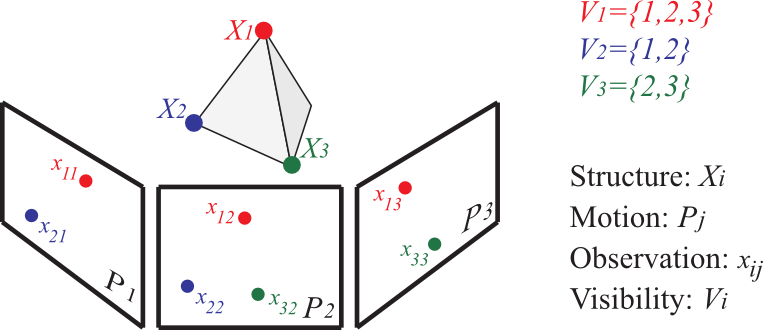
\includegraphics[width=0.45\textwidth]{images/BA.png}
 \caption{Three points $X_1, X_2, X_3$ are observed by three cameras $P_1, P_2, P_3$.}
 \label{fig:BA}
\end{figure}


\subsection{Triangulation}
TODO...

\subsection{Camera resection}
TODO...





\section{Synthetic data}

TODO...



\chapter{Technical background}
\label{cha:technical_background}

In this chapter, a briefly explanation of the used tools is given. Links to the official documentation is provided for further reading. This chapter does not intend to be a full documentation of each component, since their developments is very dynamic.

\section{ROS}
\label{sec:ros}

ROS provides standard \textbf{operating system} services such as hardware abstraction, low-level device control, implementation of commonly-used functionality, message-passing between processes, and package management.

The primary goal of ROS is to support code reuse in robotics research and development. ROS is a \textbf{distributed framework} of processes (aka \textit{Nodes}) that enables executables to be individually designed. These processes can be grouped into \textit{\textbf{Packages}}.

The ROS runtime ``graph'' is a peer-to-peer network of processes that are loosely coupled using the ROS communication infrastructure. ROS also implements several different styles of communication.

Summarizing ROS has two basic ``sides'':
\begin{itemize*}
 \item The operating system side ROS as described above,
 \item and a suite of user contributed packages (organized into sets of nodes) that implement functionalities such as: simultaneous localization and mapping, planning, perception, simulation.
\end{itemize*}

The main goal of this thesis is to be a \textbf{ROS calibration package}, in replacement of the old one \cite{pr2_calibration}. For further learning about ROS, an excellent documentation can be found in: \url{www.ros.org}.

\subsection{Roscpp}
\label{sec:roscpp}

Another primary ROS goal is \textit{``language independence''}: the ROS framework is easy to implement in any modern programming language. It is already implemented in:
\begin{itemize*}
 \item Python (\url{http://www.ros.org/wiki/rospy}) and,
 \item C++ (\url{http://www.ros.org/wiki/roscpp}).
\end{itemize*}

\noindent
Roscpp has been used in this thesis.


\subsection{RViz}
\label{sec:rviz}

It is a 3D visualization tool for ROS. It is used to visualize the \textbf{/tf} (section \ref{sec:tf}) and the \textbf{URDF} robot model (section \ref{sec:urdf}). It is also possible to send messages with basic shapes (cube, sphere, cylinder, arrow) to RViz. This Visual markers has been used in order to visualize the 3D points (see Figure \ref{fig:rviz}). For more information: \url{http://www.ros.org/wiki/rviz}.
\begin{figure}[!htbp]
 \centering
 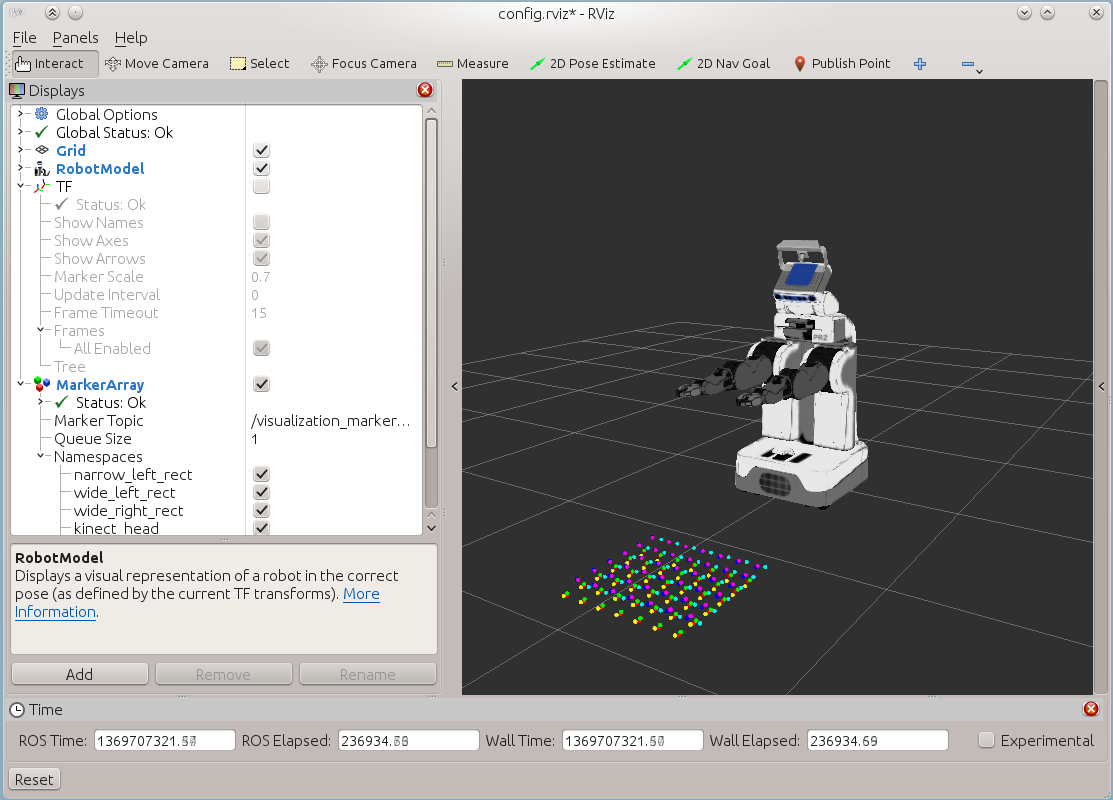
\includegraphics[width=0.95\textwidth]{images/screenshots/rviz.png}
 \caption{RViz interface.}
 \label{fig:rviz}
\end{figure}

\subsection{PR2}
\label{sec:PR2}

The PR2 (Personal Robot, version 2) is a Willow Garage which has two 7-DOF arms with a payload of 1.8 kilograms (1,800 g). Sensors include a 5 megapixel camera, a tilting laser range finder, and an inertial measurement unit. The ``texture projector'' projects a pattern on the environment to create 3D information for capture by the cameras. Also Microsoft Kinect can be head-mounted. In this work, its head (see left on Figure \ref{fig:pr2}) is the most important since all the cameras are located there and most be calibration to each other.
\begin{figure}[!htbp]
 \centering
 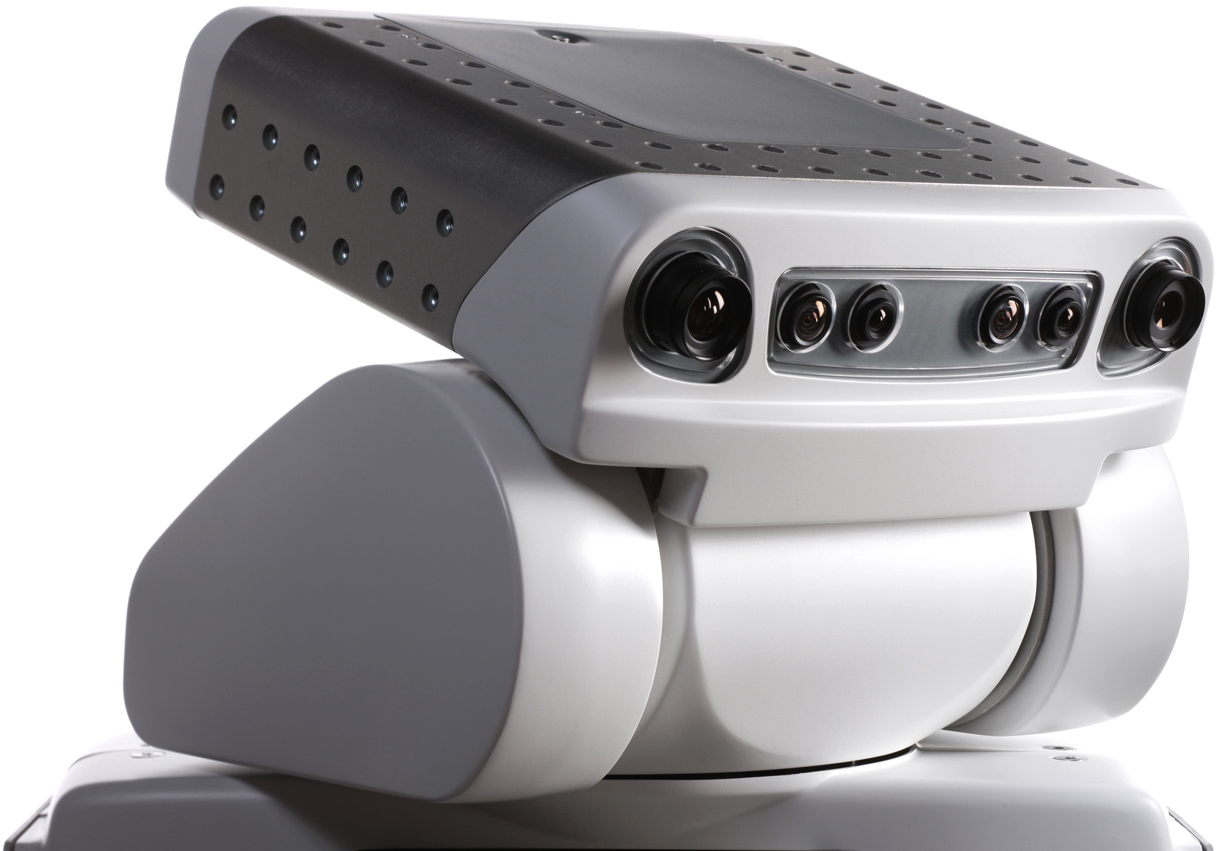
\includegraphics[width=0.45\textwidth]{images/PR2_01.jpg}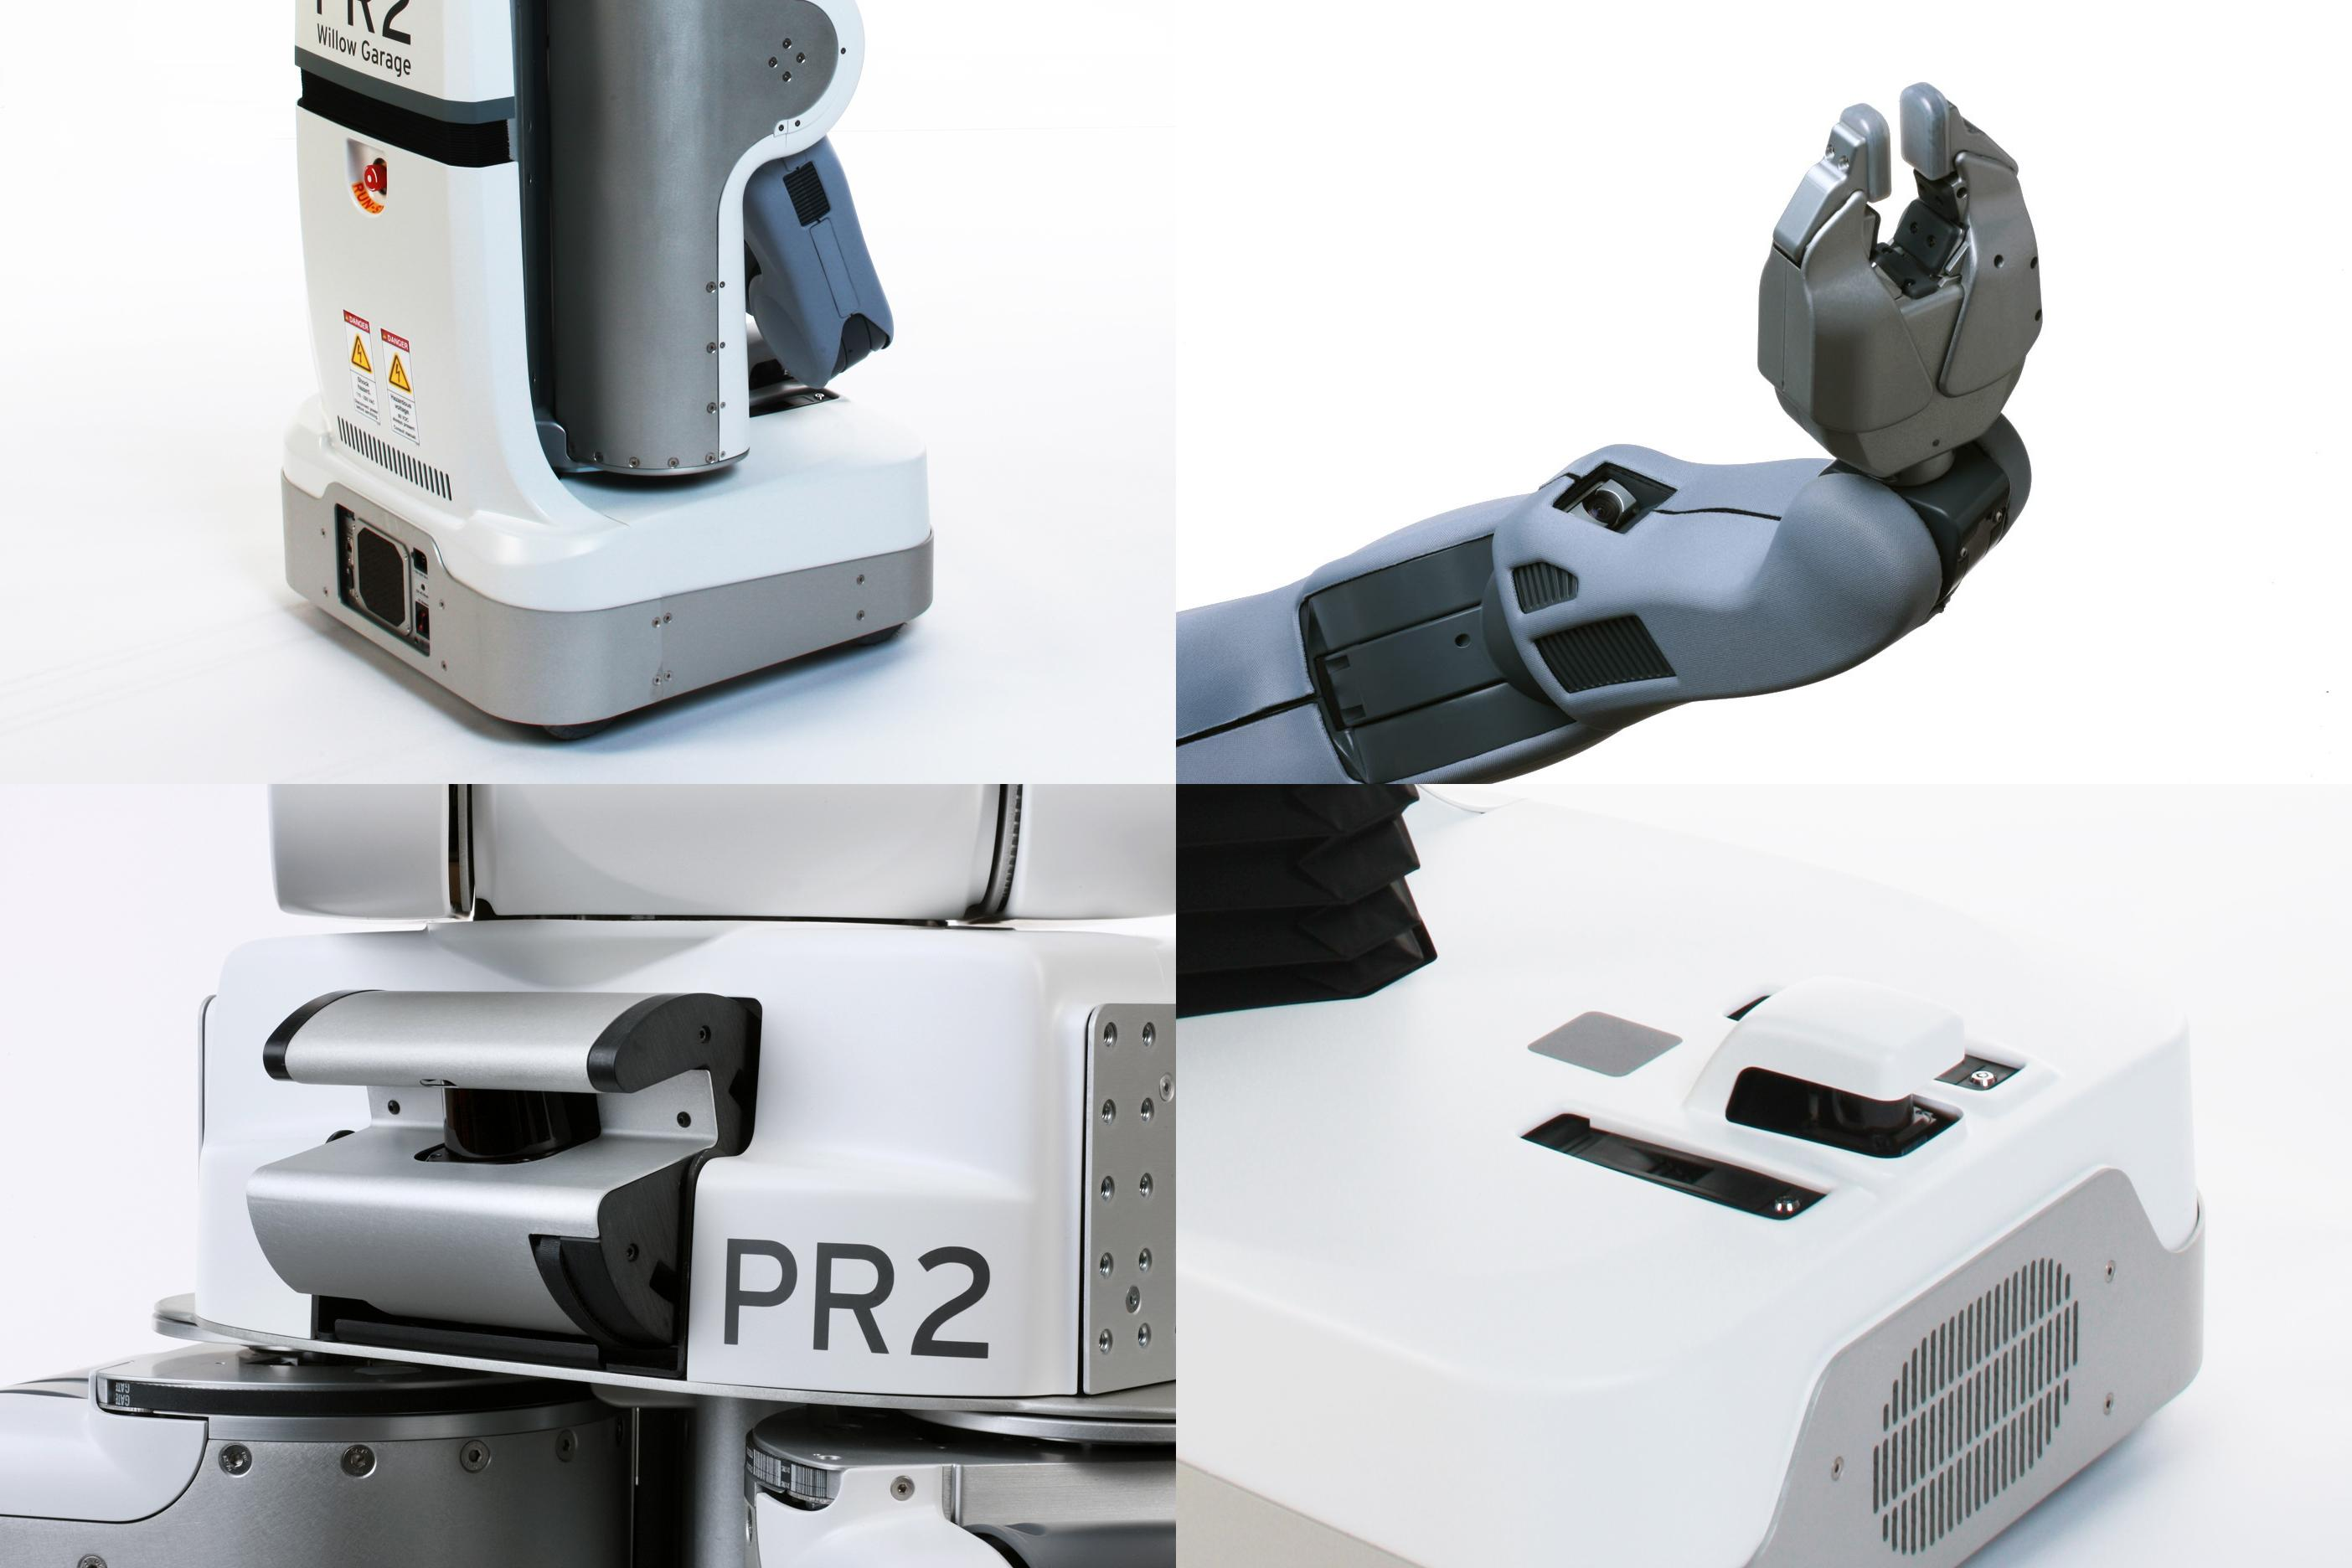
\includegraphics[width=0.45\textwidth]{images/PR2_joint.jpg}
 \caption{PR2 overview}
 \label{fig:pr2}
\end{figure}


\subsection{URDF}
\label{sec:urdf}

The URDF (\textbf{U}nified \textbf{R}obot \textbf{D}escription \textbf{F}ormat) is an XML format for representing a robot model. The package also contains a C++ parser, and it can be visualize with RViz (see in Figure~\ref{fig:pr2_urdf}).
For more information: \url{http://www.ros.org/wiki/urdf}.
\begin{figure}[!htbp]
 \centering
 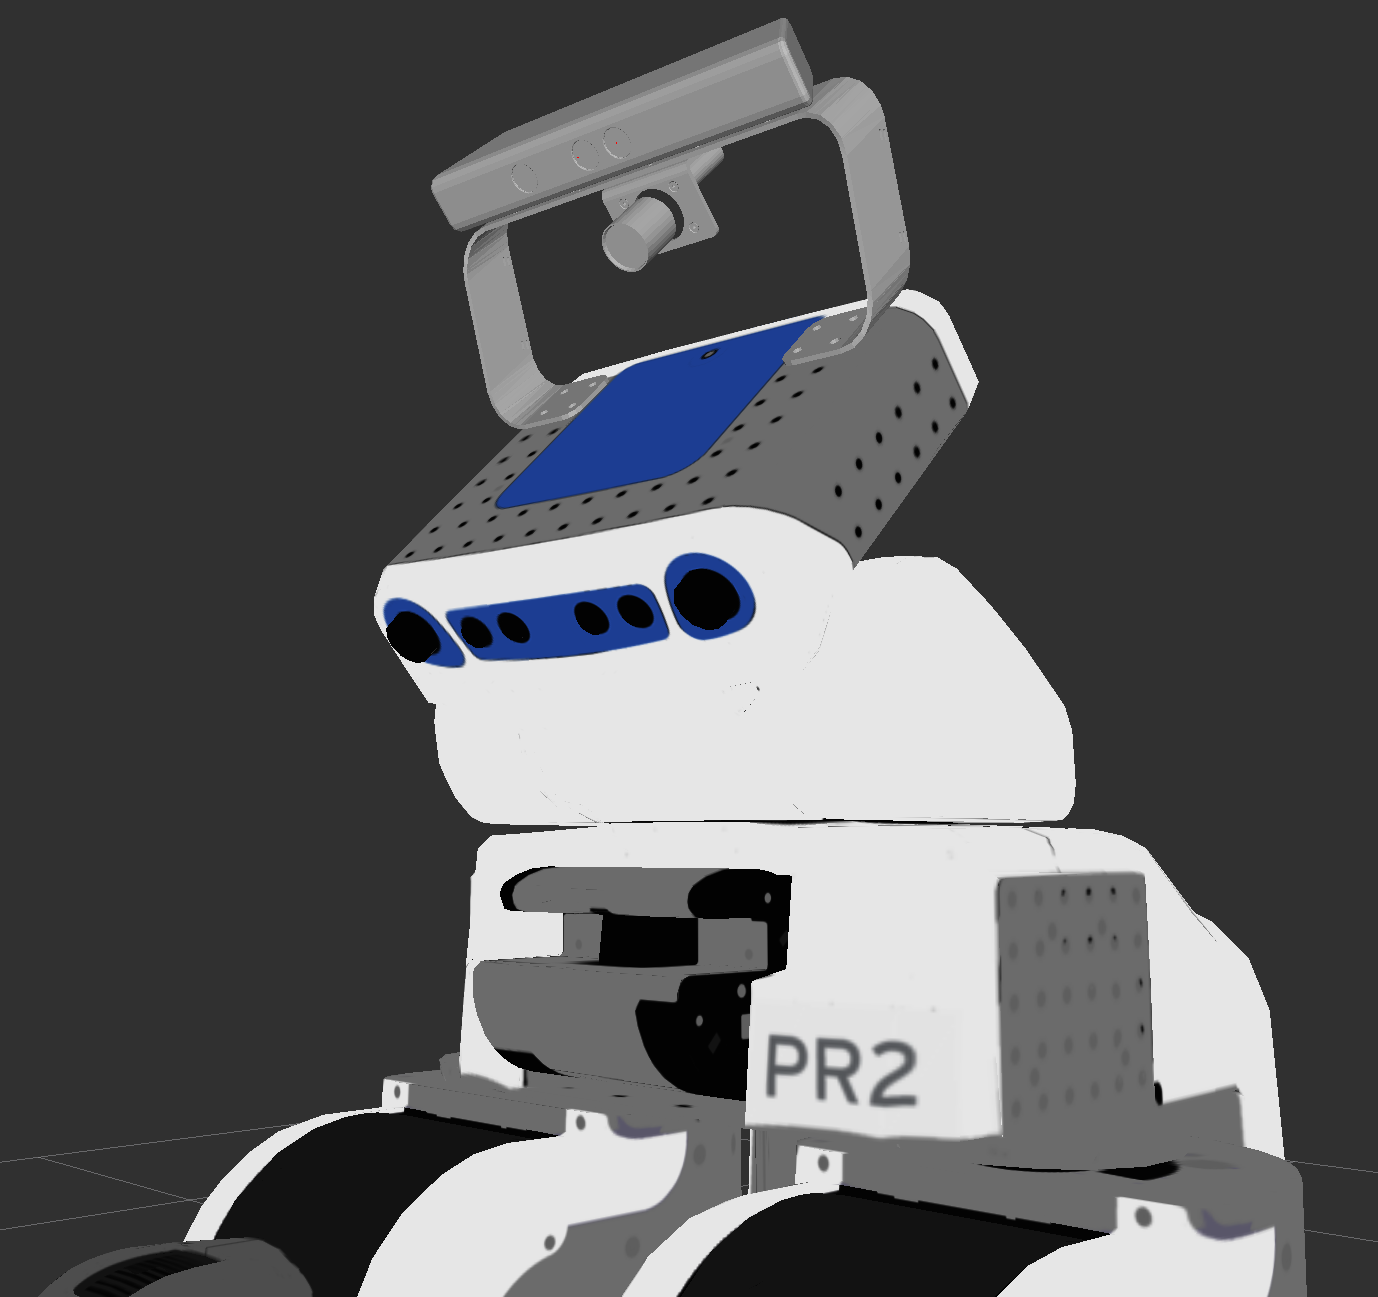
\includegraphics[width=0.35\textwidth]{images/screenshots/PR2_urdf.png}
 \caption{PR2 urdf in RViz}
 \label{fig:pr2_urdf}
\end{figure}


\subsection{/tf}
\label{sec:tf}

The package tf lets the user keep track of multiple coordinate frames over time. tf maintains the relationship between coordinate frames in a tree structure buffered in time, and lets the user transform points, vectors, etc between any two coordinate frames at any desired point in time.

A robotic system typically has many 3D coordinate frames that change over time (see Figure~\ref{fig:tf}), such as a world frame, base frame, gripper frame, head frame, etc. tf keeps track of all these frames over time.
For more information: \url{http://www.ros.org/wiki/tf}.

\begin{figure}[!htbp]
\centering
  \subfigure%[All coordinates system]
  {
    \centering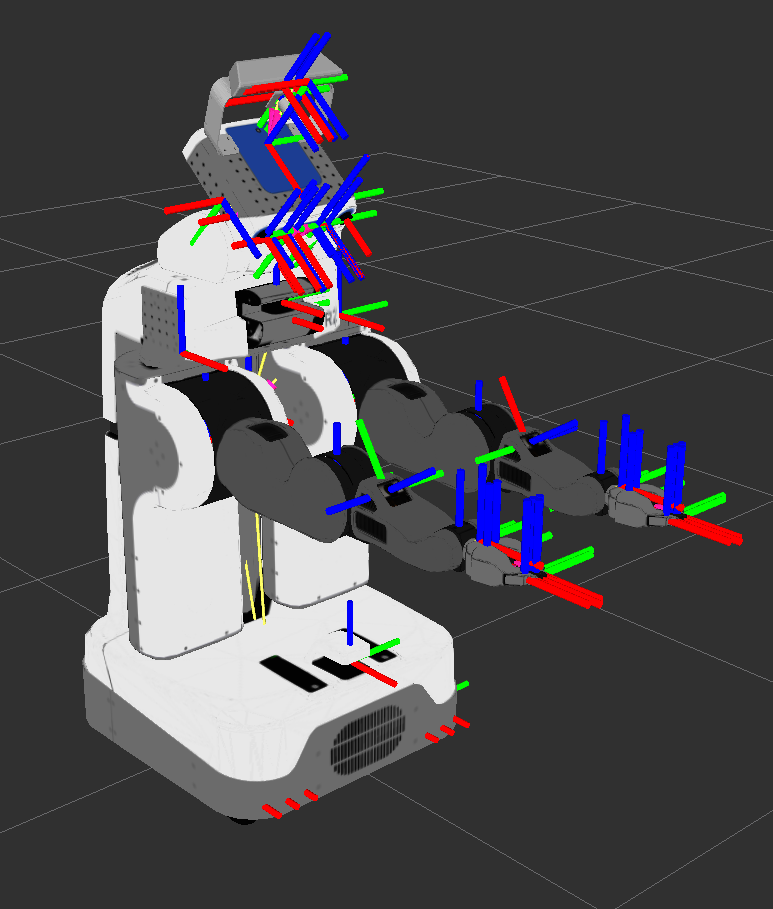
\includegraphics[height=0.3\textheight]{images/screenshots/tf01.png}
    \label{fig:tf01}
  }
  \subfigure%[\texttt{narrow\_stereo\_optical\_frame} until root]
  {
    \centering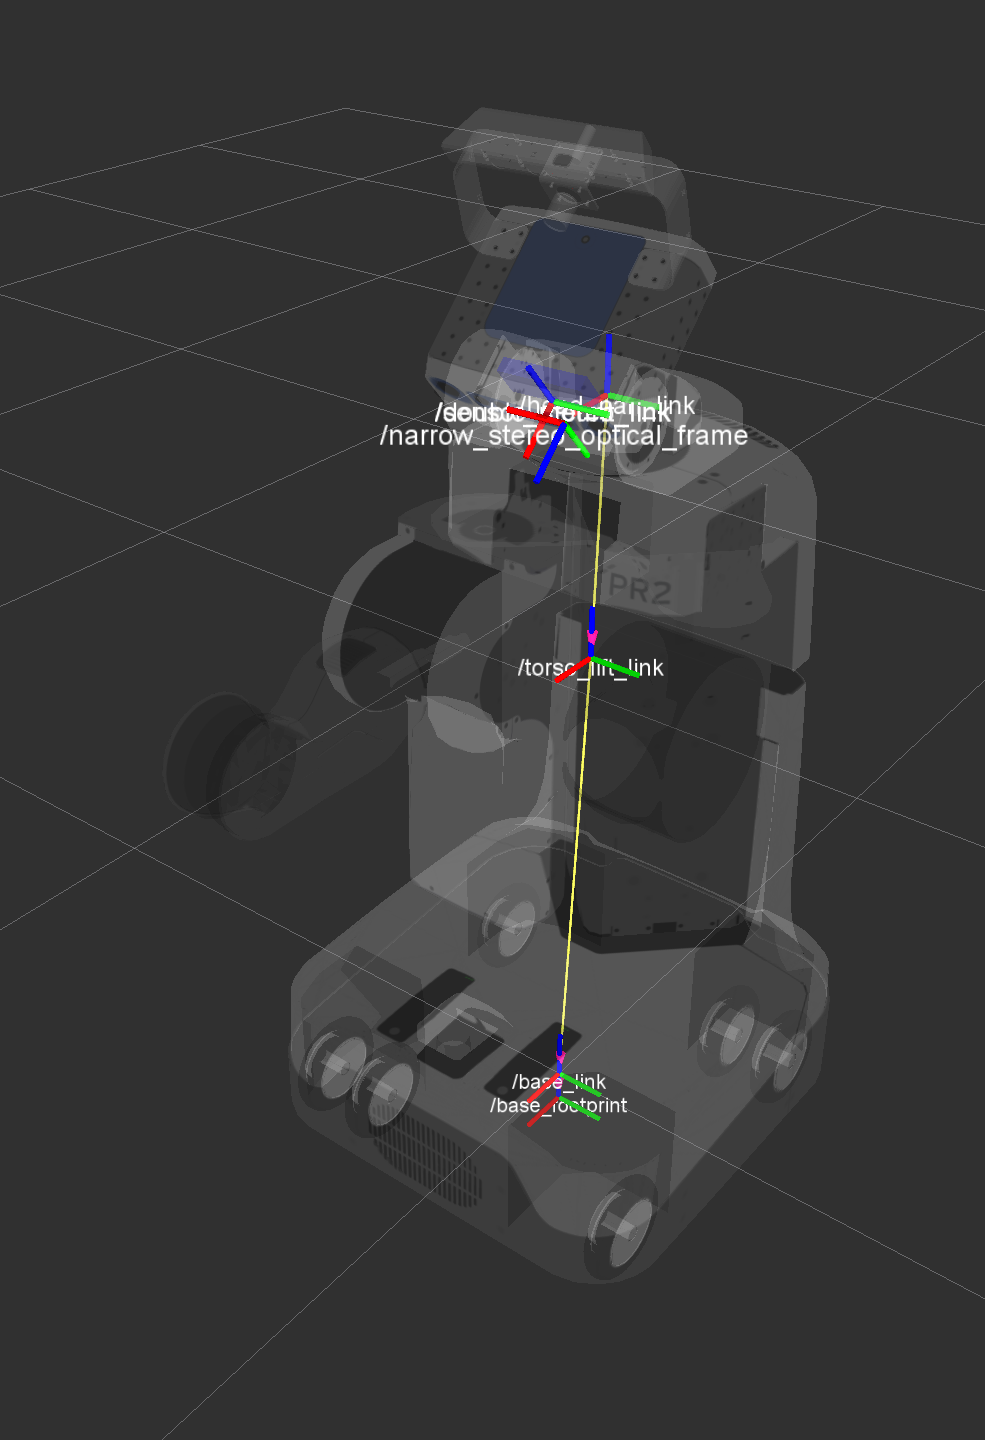
\includegraphics[height=0.3\textheight]{images/screenshots/tf02.png}
    \label{fig:tf02}
  }
  \caption{Example of /tf in RViz (in a particular time). On the left, all coordinates system; on the right, /tf path from \texttt{narrow\_stereo\_optical\_frame} until the robot root (\texttt{base\_footprint}).}
   \label{fig:tf}
\end{figure}


\subsection{ROS bag and rqt}
\label{sec:rosbag}

All the components for a simulated environment are done, and only is needed a way to reproduce events/messages. This is done with ROS bag, which is a set of tools for recording from and playing back to ROS topics. It avoids deserialization and reserialization of the messages. More info: \url{http://www.ros.org/wiki/rosbag}.

\begin{figure}[!htbp]
 \centering
 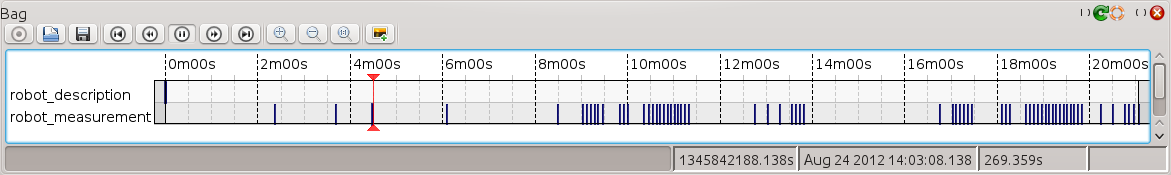
\includegraphics[width=0.95\textwidth]{images/screenshots/rosbag01.png}
 \caption{rqt: \rosbag~interface.}
 \label{fig:rosbag01}
\end{figure}

A second tool described here is a rqt plugin which allows to play a ROS bag easily (Figure~\ref{fig:rosbag01}). The user will be able to see the ROS messages in a convenient way (Figure~\ref{fig:rosbag02}). More info: \url{http://www.ros.org/wiki/rqt}.

\begin{figure}[!htbp]
 \centering
 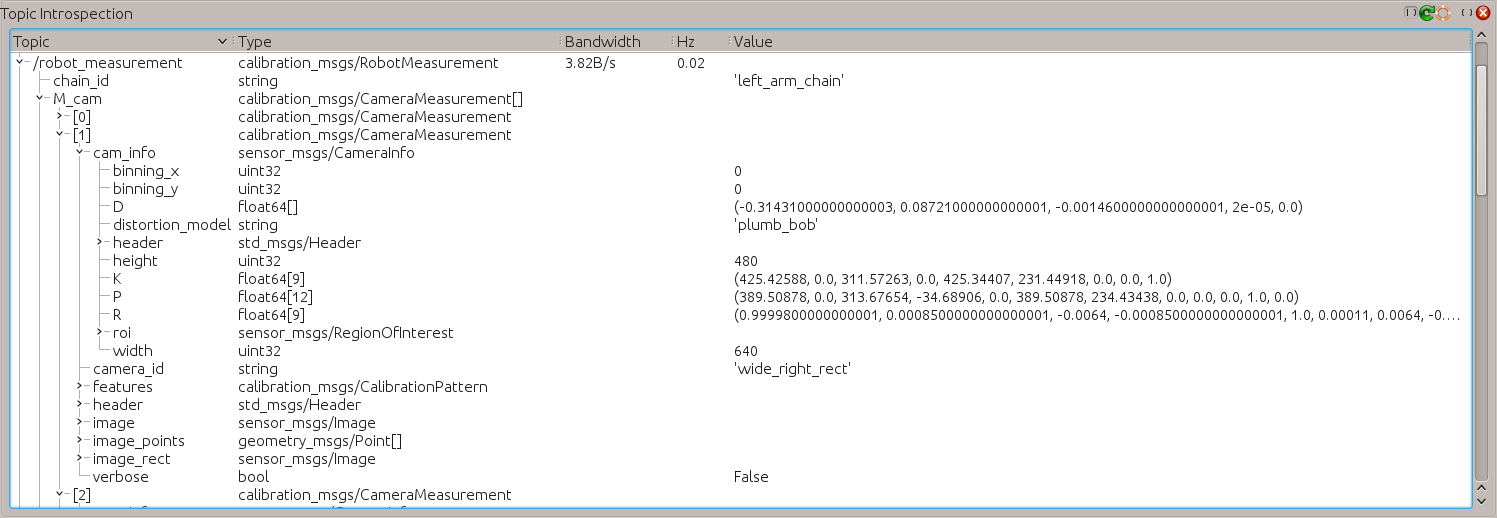
\includegraphics[width=0.95\textwidth]{images/screenshots/rosbag02.png}
 \caption{rqt: Topic introspection.}
 \label{fig:rosbag02}
\end{figure}


\section{KDL}
\label{sec:KDL}

KDL (\textbf{K}inematics and \textbf{D}ynamics \textbf{L}ibrary) defines a tree structure to represent the kinematic and dynamic parameters of a robot mechanism (see Figure \ref{fig:KDL}). \textit{kdl\_parser} provides tools to construct a KDL tree from an XML robot representation in URDf format.

\begin{figure}[!htbp]
 \centering
 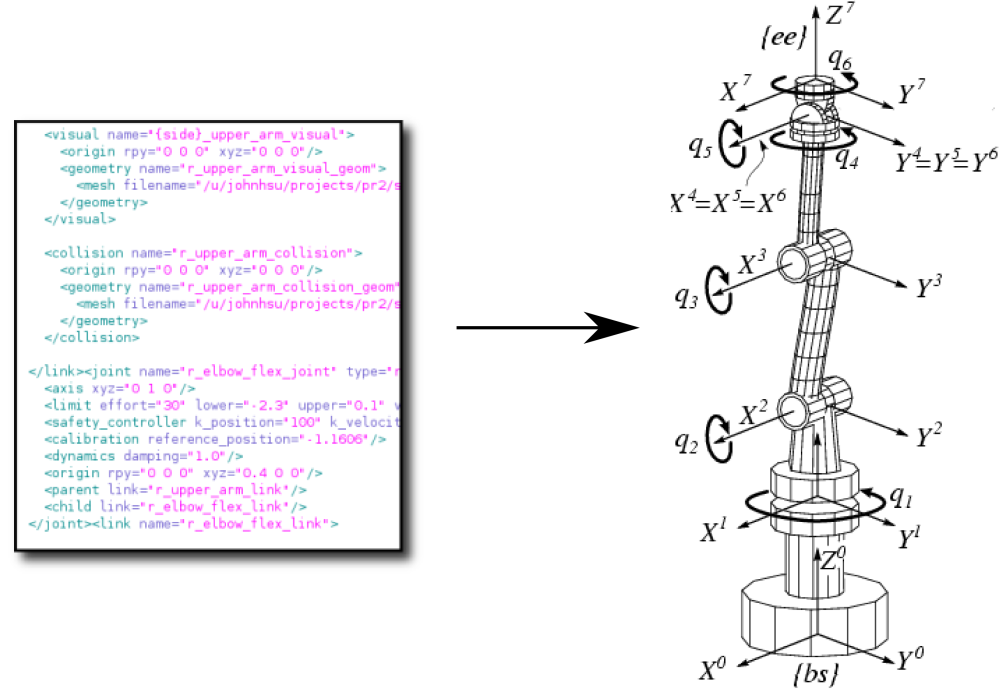
\includegraphics[width=0.7\textwidth]{images/KDL02.png}
 \caption{Example of KDL tree.}
 \label{fig:KDL}
\end{figure}

This library is mainly used for:
\begin{itemize*}
 \item 3D frame and vector transformations,
 \item forward kinematics (given joint angles compute the position of the end-effector\footnote{An \textit{end-effector} is the device at the end of a robotic arm, designed to interact with the environment, in our case the cameras.}).
\end{itemize*}


For more information: \url{http://www.ros.org/wiki/kdl}.

\section{Ceres}
\label{sec:Ceres}

Ceres Solver \cite{ceres} is a portable C++ library that allows modeling and solving large complicated \textbf{non-linear least squares} problems. It is used at Google to estimate the pose of Street View cars, aircrafts, and satellites; to build 3D models for PhotoTours; to estimate satellite image sensor characteristics, and more.

Ceres Solver is an important component in this thesis because, among others, it has very good features like:
\begin{itemize*}
\item A friendly API: build your objective function one term at a time.
\item Automatic Analytic Derivatives.
\item Specialized solvers for bundle adjustment problems in computer vision.
% \item Iterative linear solvers for general sparse and bundle adjustment problems.
\end{itemize*}

It will too long to make a good introduction to Ceres, but a briefly description of important points, obtained from the tutorial, can be found in the following. The excellent tutorial is available in: \url{http://homes.cs.washington.edu/~sagarwal/ceres-solver/tutorial.html}.

\subsection*{Modeling}
Ceres solves robustified non-linear least squares problems of the form:
\[
\frac{1}{2}\sum_{i=1} \rho_i\left(\left\|f_i\left(x_{i_1}, ... ,x_{i_k}\right)\right\|^2\right).
\]

The expression $\rho_i\left(\left\|f_i\left(x_{i_1},...,x_{i_k}\right)\right\|^2\right)$ is known as a \texttt{ResidualBlock}, where $f_i(\cdot)$ is a \texttt{Cost Function} that depends on the parameter blocks $\left[x_{i_1},... , x_{i_k}\right]$. In most optimization problems small groups of scalars occur together. For example, the three components of a translation vector and the four components of the quaternion that define the pose of a camera. We refer to such a group of small scalars as a \texttt{ParameterBlock}. Of course a \texttt{ParameterBlock} can just be a single parameter.

$\rho_i$ is a \texttt{LossFunction}. A \texttt{LossFunction} is a scalar function that is used to reduce the influence of outliers on the solution of non-linear least squares problems. As a special case, when $\rho_i(x) = x$, i.e., the identity function, we get the more familiar non-linear least squares problem.
\[
 \frac{1}{2}\sum_{i=1} \left\|f_i\left(x_{i_1}, ... ,x_{i_k}\right)\right\|^2.
\]

\subsection*{Derivatives}
Ceres Solver like most optimization packages, depends on being able to evaluate the value and the derivatives of each term in the objective function at arbitrary parameter values. Doing so correctly and efficiently is essential to getting good results. Ceres Solver provides a number of ways of doing so: Analytic and Numeric Derivatives. In order to use Automatic differentiation, it is necessary to define a \textbf{templated} cost functor\footnote{A functor is a class with an \texttt{operator()} member. And a cost functor is a functor which evaluate the residuals.}.



\chapter{Multi-view recalibration}
\label{cha:multi-view calibration}

\vspace*{-3ex}
The relation between the tools previously defined is provided here, explaining the way they work together in both the acquisition and estimation process.

This chapter is divided in three main sections: \textbf{acquisition}, \textbf{visualization} and \textbf{estimation}. Recall that the goal is to recalibration multiple cameras, using the PR2 as a real example, and focused in the estimation part.

\section{Overview}
\label{sec:estimation_overview}

In Figure \ref{fig:high_level_flow} a high level chart flow is presented: \textbf{1.} camera measurements are collected (checkerboard corners, as explained in section \ref{sec:acquisition}); \textbf{2.} then estimation process is optimizing a non-linear function in order to estimate the cameras poses; \textbf{3.} publishing the result to \texttt{/tf}.

\begin{figure}[!htbp]
 \centering
 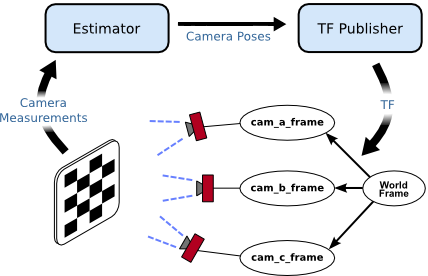
\includegraphics[width=0.5\textwidth]{images/high_level_flow_02.png}
 \caption{High level flow.}
 \label{fig:high_level_flow}
\end{figure}

\noindent
\textbf{Note}: point \textbf{3.} is optional. Since it was desired a visual feedback for the estimation process, it was necessary to considered this option from the beginning in the design. An alternative to \textbf{3.} is to save the result as a new and unique URDF for the particular robot it is being calibrated.



\subsection*{Preliminary: cameras in the PR2}

The PR2 has 6 cameras in its head:
\begin{itemize*}
 \item 2 narrow range. Topics: \texttt{wide\_right\_rect} and \texttt{wide\_left\_rect}.
 \item 2 wide range. Topics: \texttt{narrow\_right\_rect} and \texttt{narrow\_left\_rect}.
 \item 1 Kinect. Topic: \texttt{kinect\_head}.
 \item 1 High definition. Topic: \texttt{Prosilica\_rect}.
\end{itemize*}

\noindent
The initial camera configuration can be seen in Figure \ref{fig:pr2_cameras}, provided by the URDF. \textbf{Note}: this is the initialization and the information to be calibrated.
\begin{figure}[!htbp]
 \centering
 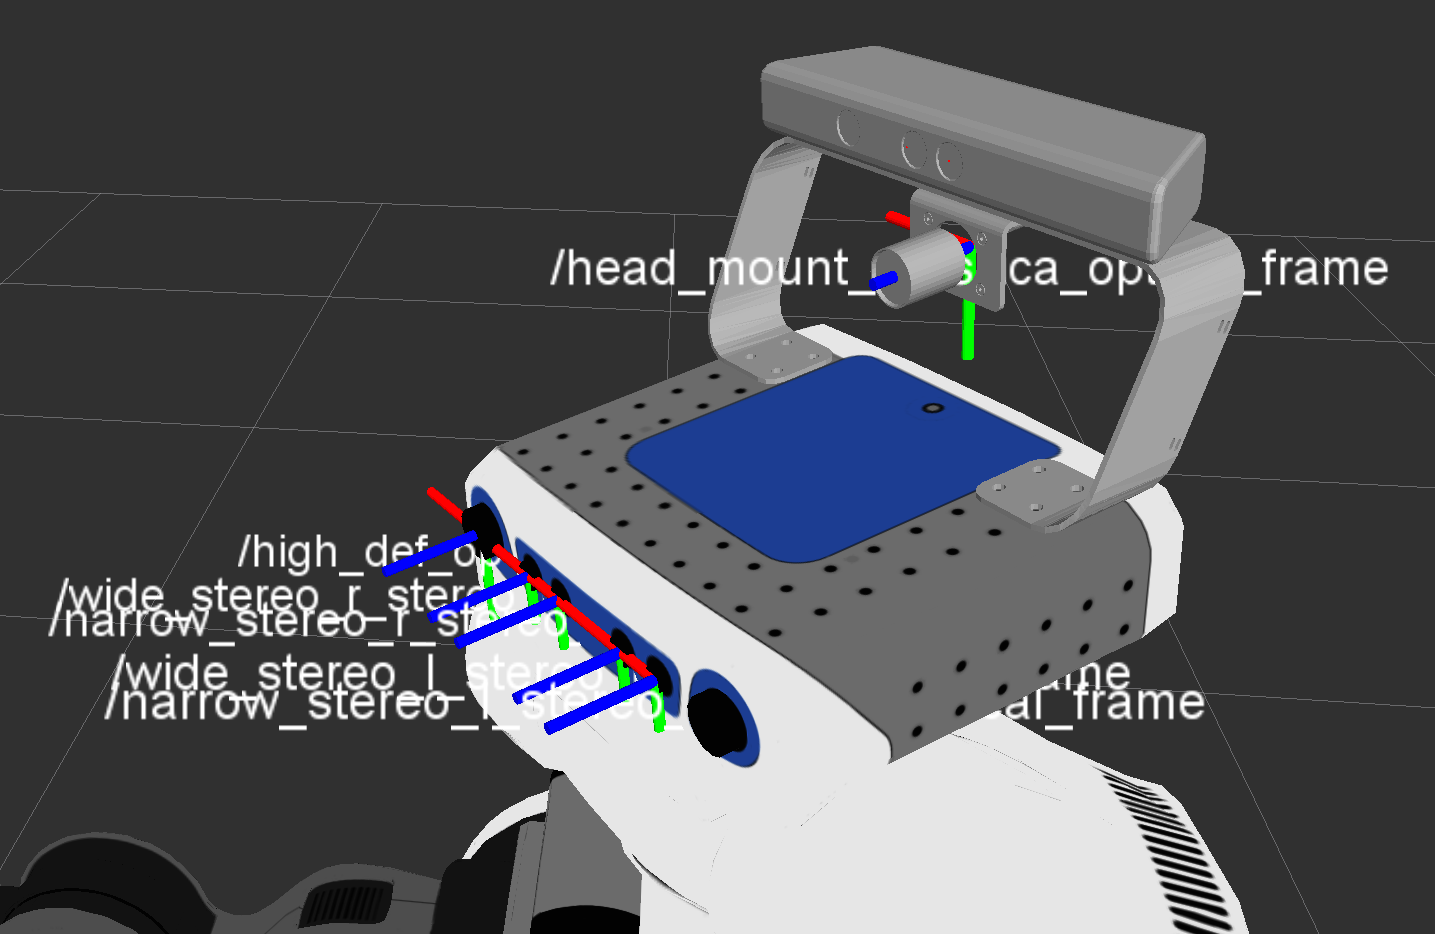
\includegraphics[width=0.55\textwidth]{images/screenshots/PR2_cameras.png}
 \caption{Coordinate system of all the cameras in the PR2 head.}
 \label{fig:pr2_cameras}
\end{figure}






\section{Acquisition process}
\label{sec:acquisition}

This is the \textit{point \textbf{1.}} in the overview (Figure \ref{fig:high_level_flow}). The acquisition part was already implemented, and a full description can be found in the paper  \cite{pr2_calibration_paper} and in the ROS tutorials for the PR2 calibration package.

% The thesis is focused in the estimation part but, in order to reach part, it is necessary first to do some comments regarding the process and
%
% % In the paper  and the ROS tutorials for the PR2 calibration package, the full description of the acquisition process will
% In this section will explain the acquisition process. It will explain


\subsection{Data collection}

In order to sufficiently constrain the non-linear optimization (see \cite{pr2_calibration_paper}), it is needed to collect a large amount of data, and manually collecting this calibration data can be tedious. By having the PR2 hold a checkerboard in its gripper (Figure~\ref{fig:pr2_holdind_cb}), a total of 30 checkerboard poses measurements are collected for each hand. Also, 4 samples of a \textbf{large checkerboard} that is far from the robot in order to help with far-field calibration (see Figure \ref{fig:data_collection01}). This data is saved in a ROS bag (section~\ref{sec:rosbag}) and posteriorly processed for the calibration package.

\noindent

\textbf{Notes}:
\begin{itemize*}
  \item It is important to mention at this point the 2D measurements are obtained from rectified images (section \ref{sec:rectification}). Therefore, working with distortion is happily avoided in the estimation process.
  \item It is assumed all cameras have been intrinsically calibrated in a previous stage.
\end{itemize*}


\begin{figure}[!htbp]
  \centering
  \raisebox{2ex}{
    \subfigure
    {
      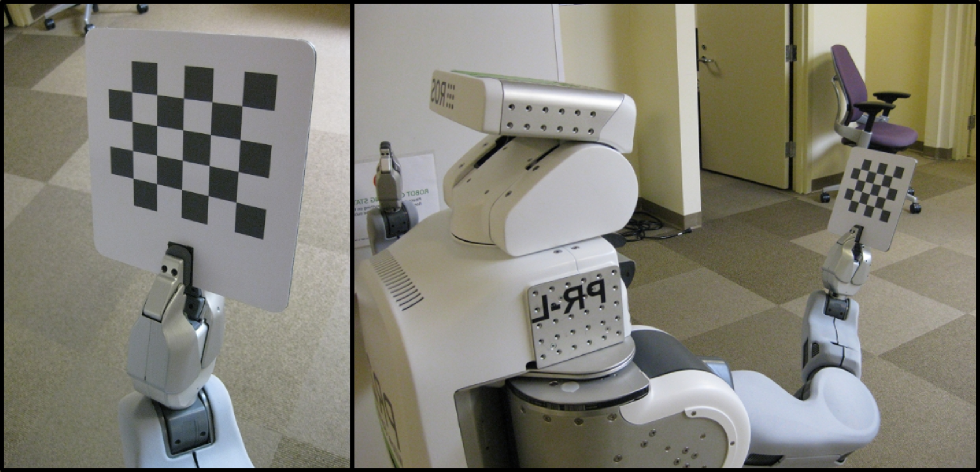
\includegraphics[width=0.5\textwidth]{images/pr2_holdind_cb.png}
    }
  }
  \subfigure
  {
    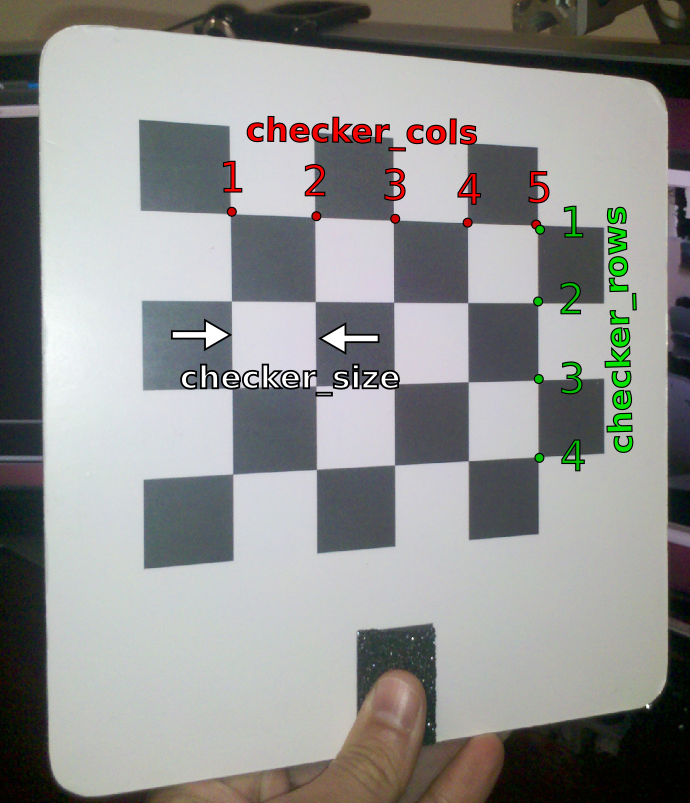
\includegraphics[width=0.25\textwidth]{images/checkerboard01.png}
  }
  \caption{The PR2 holding a checkerboard pattern.}
 \label{fig:pr2_holdind_cb}
\end{figure}


\begin{figure}[!htbp]
 \centering
 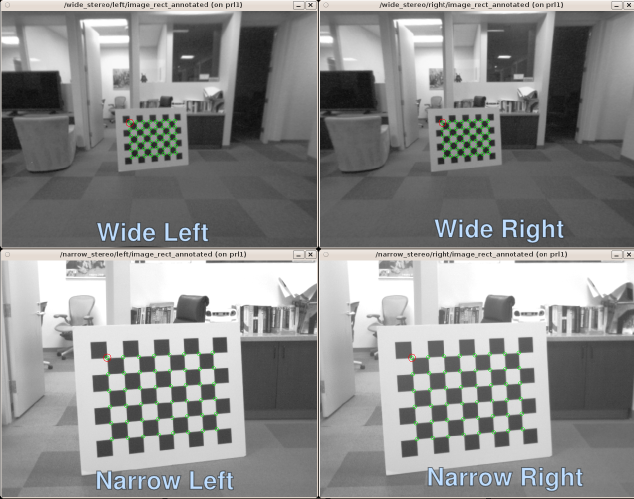
\includegraphics[width=0.7\textwidth]{images/data_collection01.png}
 \caption{Example of \textit{one} sample from 4 different view, using the large checkerboard.}
 \label{fig:data_collection01}
\end{figure}




\section{Visualization}
\label{sec:visualization}

This is the \textit{point \textbf{3.}} in the overview (Figure \ref{fig:high_level_flow}). This part is optional, but it was crucial to understand what was happening and to debug problems and solutions.

Even though publishing to /tf is not difficult to do, it has been time consuming and more details will be given in chapter \ref{cha:implementation}. %, where implementation details are given\footnote{Publish to /tf is mentioned here to be consistent with the overview.}.

For now, let's us concentrate in 3D points visualization, more precisely RViz Markers.

\subsection{Visual Markers}
\label{sec:visual_markers}

Since checkerboards are seen from multiple views, an idea to check if the system is calibrated is to overlap the 3D obtained from individuals cameras using solvePnP, described in section \ref{sec:solvePnP}. Two examples can be seen in Figure \ref{fig:visual_markers}. Different colors have been used for different cameras.

\begin{figure}[!htbp]
  \centering
  \subfigure[Checkerboard in hand.]{
    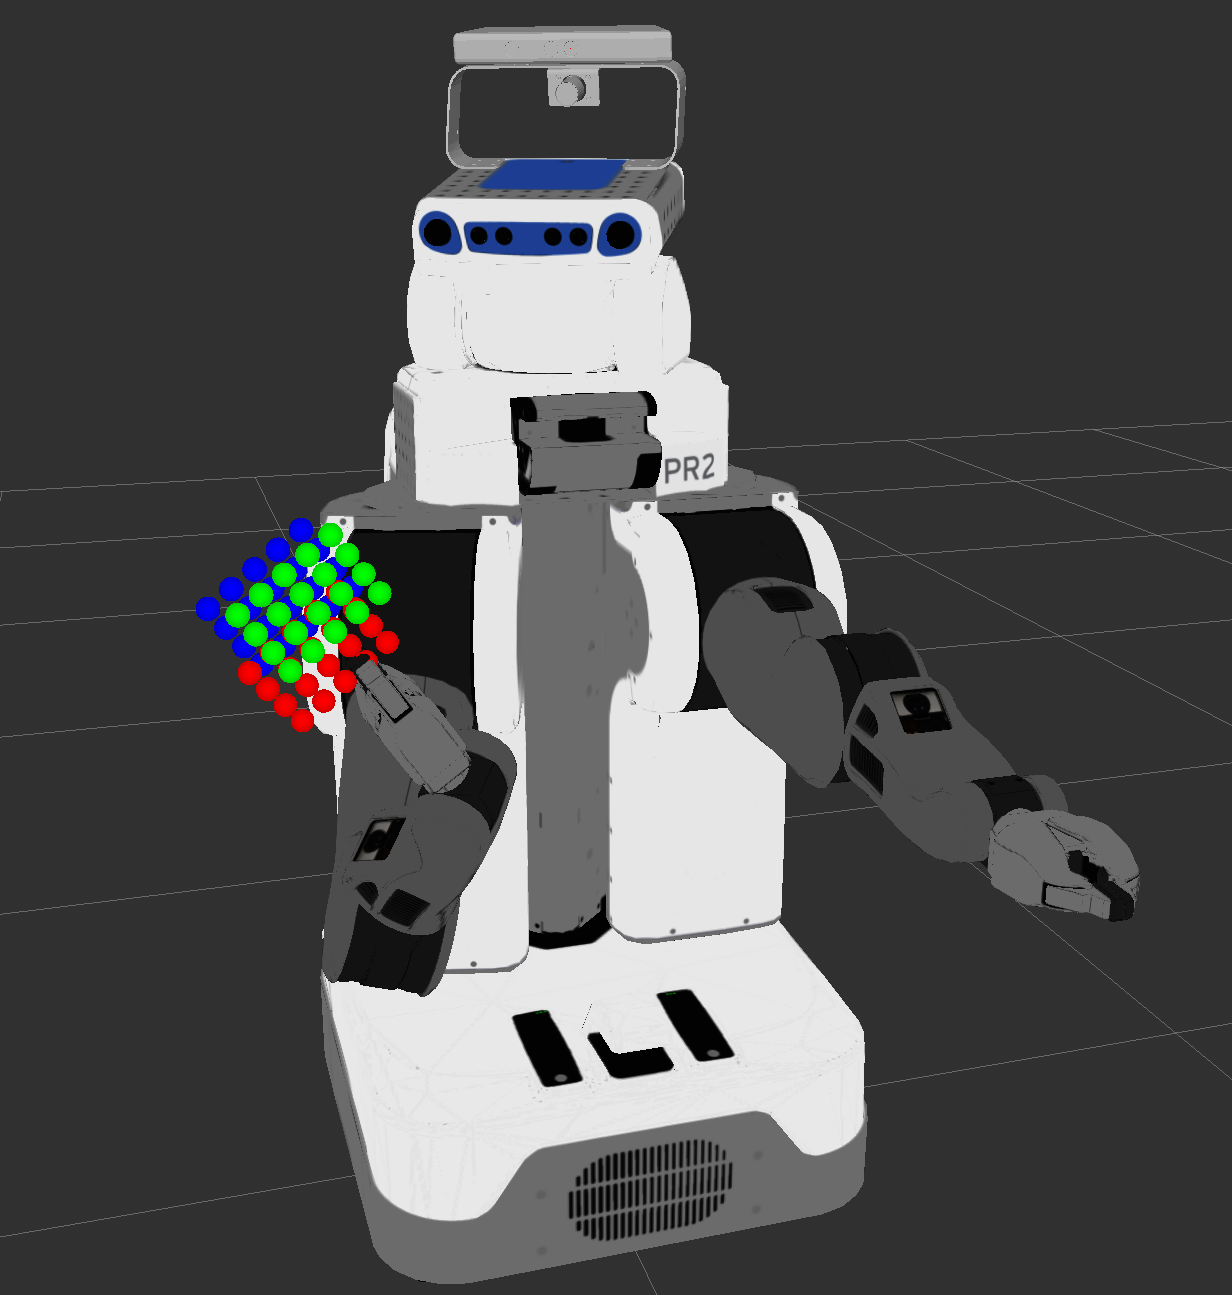
\includegraphics[height=0.35\textheight]{images/screenshots/uncalib10_1.png}
  }
  \subfigure[Checkerboard free in the world.]{
    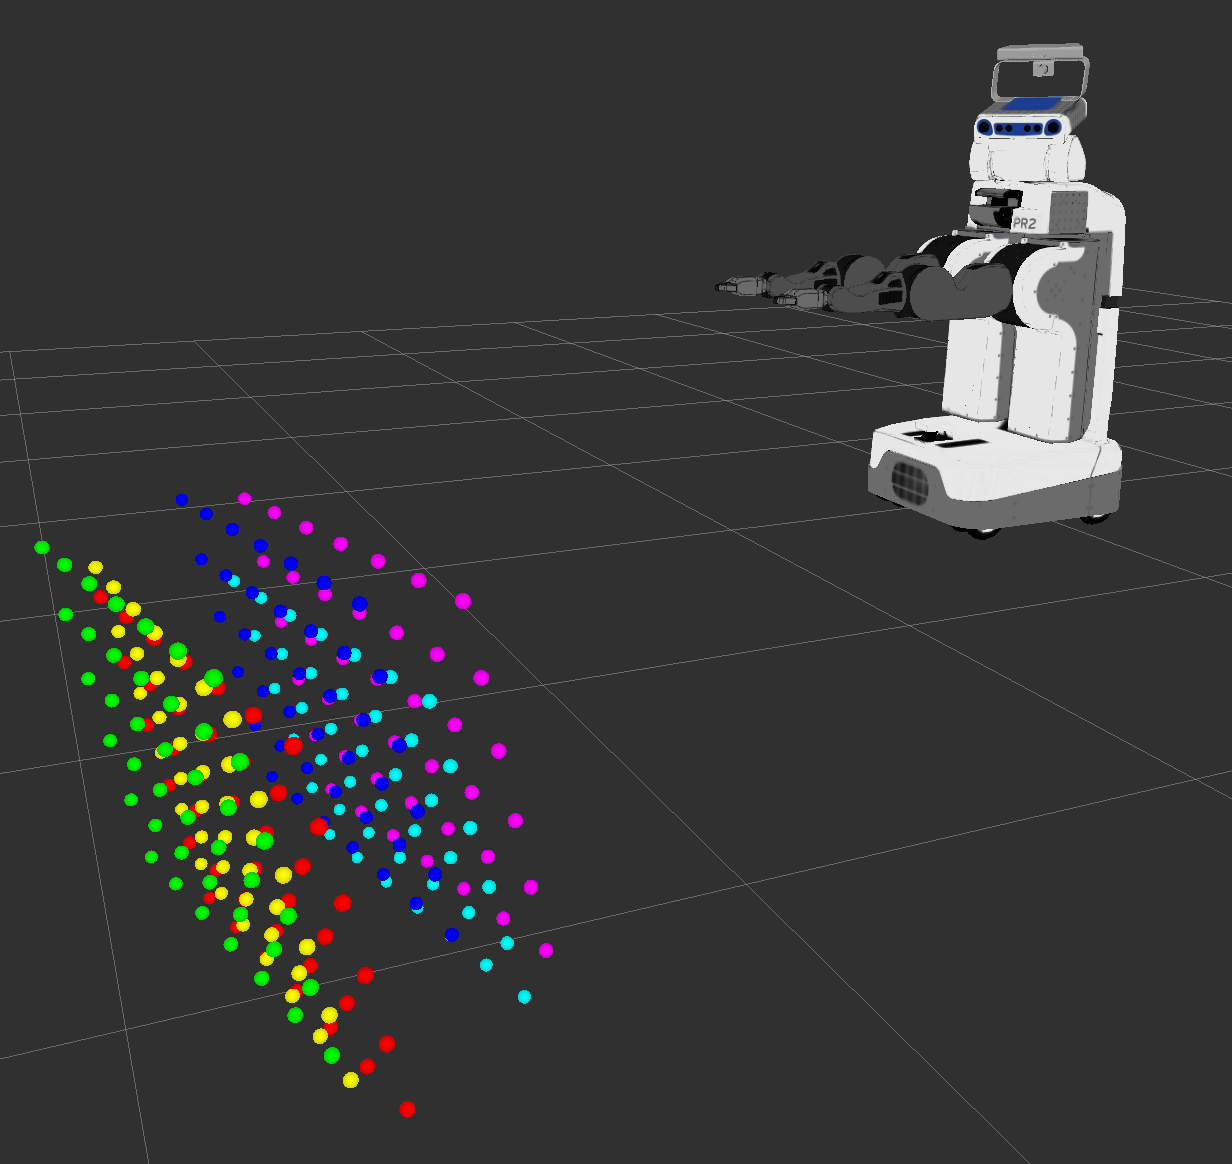
\includegraphics[height=0.35\textheight]{images/screenshots/uncalib03_1.png}
  }
  \caption{solvePnP results for the all the cameras (same checkerboard).}
  \label{fig:visual_markers}
\end{figure}

\noindent
\textbf{Note:} this is not the best approach to get 3D points since they are obtained from measurements of individual cameras. It is used here for a quick comparison, in order to see how bad the calibration is. A superior method is to use all the cameras measurements minimizing an \textit{algebraical error} (linear), the n-view triangulation method (section \ref{sec:nview_triangulation}); and followed by a \textit{geometrical error} minimization (non-linear), the re-projection error. It is superior because it is optimal in the \textbf{maximum likelihood} sense.

\section{Estimation process}
\label{sec:estimation}

This is the \textit{point \textbf{2.}} in the overview (Figure \ref{fig:high_level_flow}).
The estimation process is divided in turn in three stages: \textbf{initialization}, actual \textbf{optimization} and \textbf{updating} URDF robot model with the results (see Figure \ref{fig:optimization}).

\begin{figure}[!htbp]
 \centering
 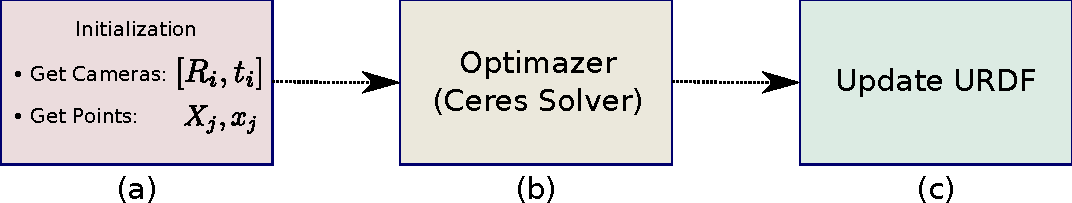
\includegraphics[width=0.7\textwidth]{images/optimization.pdf}
 \caption{Estimation process.}
 \label{fig:optimization}
\end{figure}

% Needing to estimate relative poses of several cameras or many poses of a single moving camera is a somewaht common problem. It is often solve by jointly estimating the set of camera poses along with 3D features that are detected by some set of cameras. This approach is called bundle adjustment \cite{BA}.
%
% We have in condition now explain the estimation process, all the needed components have been explained.


\subsection{Initialization}

\subsubsection*{Get cameras}

An \textbf{initial configuration} of the cameras is given by the URDF, it comes from the robot design.

Since PR2 head moves in the data collection, the camera poses change with respect to the robot coordinate system in each calibration step, depending of the angles joints. Them, \textbf{forward kinematics} is needed and KDL (section \ref{sec:KDL}) is extremely useful here.
\textbf{Note}: even though the robot moves, the relative position of the cameras does not change, it is a rigid relationship between them since they are all located in head which is a whole entity.

\begin{figure}[!htbp]
 \centering
 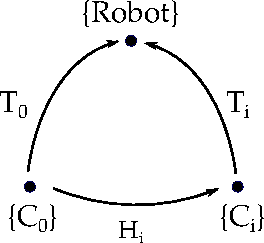
\includegraphics[width=0.3\textwidth]{images/initialization.pdf}
 \caption{Relative transformations.}
 \label{fig:initialization}
\end{figure}

\noindent
In order to understand Figure \ref{fig:initialization}, some terms are introduced below:
\begin{itemize*}
 \item[-] \{\textbf{Robot}\}: robot coordinate system. It is the root of the URDF tree, usually called \texttt{base\_footprint} link.

 \item[-]  \{$\mathbf{C_i}$\}: camera coordinate system $i$. The \textit{reference camera} is $C_0$.

 \item[-]  \{$\mathbf{T_i}$\}: transformation from  \{$\mathbf{C_i}$\} to \{\textbf{Robot}\}.

 \item[-] \{$\mathbf{H_i}$\}: transformation from  \{$\mathbf{C_0}$\} to  \{$\mathbf{C_i}$\}. It is the relative position between them, from rotation and translation matrices are obtained.
\end{itemize*}

% \noindent
Then,
\begin{equation}
 H_i = T_i^{-1} \, T_0
\end{equation}

rotation $R_i$ and translation $t_i$ of the camera $i$ can be extracted from $H_i$,
\begin{equation}
 H_i = \begin{pmatrix}
        R_i & t_i \\
        0   & 1
        \end{pmatrix}
\end{equation}

\subsubsection*{Get points}

Now, 3D points should be obtained from the measurements as an initialization. Two initialization are possibles:
\begin{itemize*}
 \item using \textbf{solvePnP} (section \ref{sec:solvePnP}) in the reference camera, 3D points will minimize re-projection error in the first camera. This is not an optimal initialization, as it is explained in the end of section \ref{sec:visualization},

 \item using \textbf{n-view triangulation} (section \ref{sec:nview_triangulation}): by the moment of writing the thesis, this part is considered as ``\textit{work in progress}'', therefore results of this initialization are not provided, more details of the problems encountered are explained in the implementation chapter \ref{cha:implementation}. Note: it is a natural extension of the triangulation method, which minimize an algebraical error. This could be a better initialization for the structure in comparison with the previous one.
\end{itemize*}



\subsubsection*{Get projection matrices}

As it stated in section \ref{sec:BA}, BA takes \textbf{measurements}, \textbf{3D Points} (structure) and \textbf{projection matrices}~$P_i$. The last step needed here is to multiply $[R_i ~~ t_i]$ by $K_i$ (camera intrinsic matrix), and it is assumed to have this information. Then,
\[
 P_i = K_i \, [R_i ~~ t_i]
\]




\subsection{Per view optimization}

In order to test the system before going to the complete optimization (optimizing the parameters with data in all views), a ``local'' per view optimization (only one checkerboard sample) was performed to see if the process was going in the right path. This previous stage before using all the data was important to find errors.

TODO... Move to implementation chapter!!



\subsection{Optimizer}

This part will be considered in the implementation chapter (section \ref{sec:ceres_impl}).


\subsection{Update URDF}

TODO....



------------------


\subsection{Results}
\label{sec:results}

In this section, a visual comparison is given. First, result before and after optimization process are compared visually using solvePnP as is described in section \ref{sec:visual_markers}. Second, a quantitative comparison of the optimization process output is provided.

\subsubsection{Visual comparison}

Only two of a total of 64 checkerboard samples are shown here: checkerboard in hand in Figure \ref{fig:cal_hand}, and checkerboard free in the world in Figure \ref{fig:cal_free}. It is possible to appreciate that after the optimization process the checkerboards are more close each others, indicating it is a better calibration has been obtained, next section gives a more exhaustive comparison of the estimation process results.
% it does not mean it is a good one.
%

\begin{figure}[!htbp]
 \centering
   \subfigure[Before estimation.]
   {
      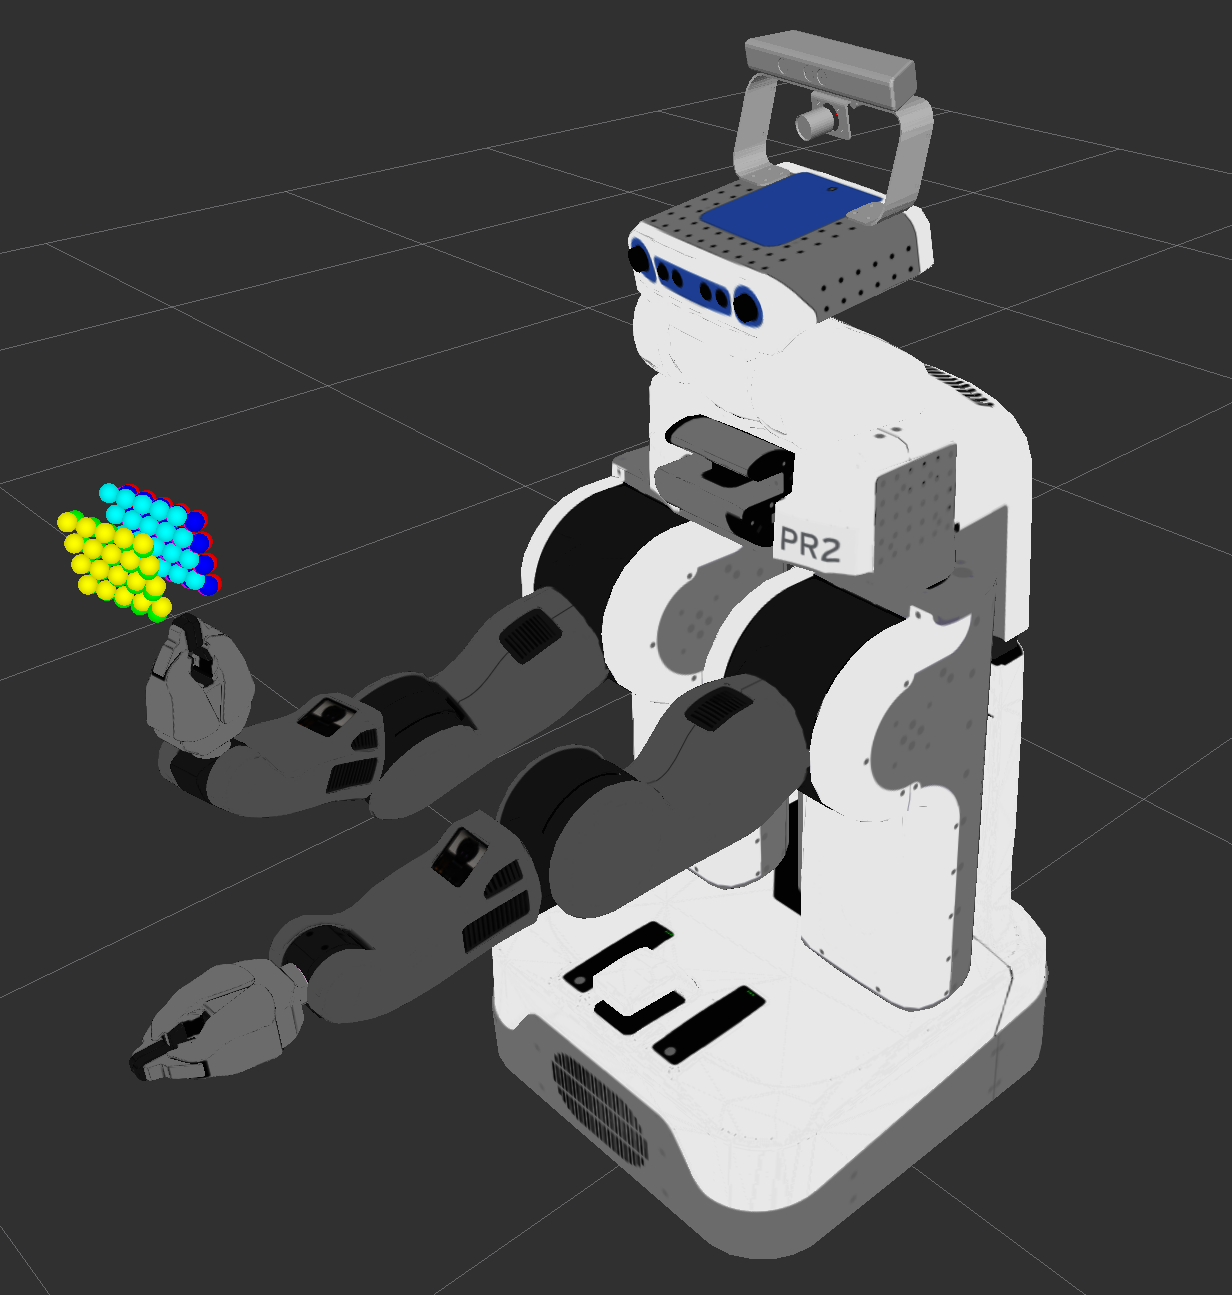
\includegraphics[height=0.25\textheight]{images/screenshots/uncalib08_1.png}
   }
   \subfigure[After estimation.]
   {
      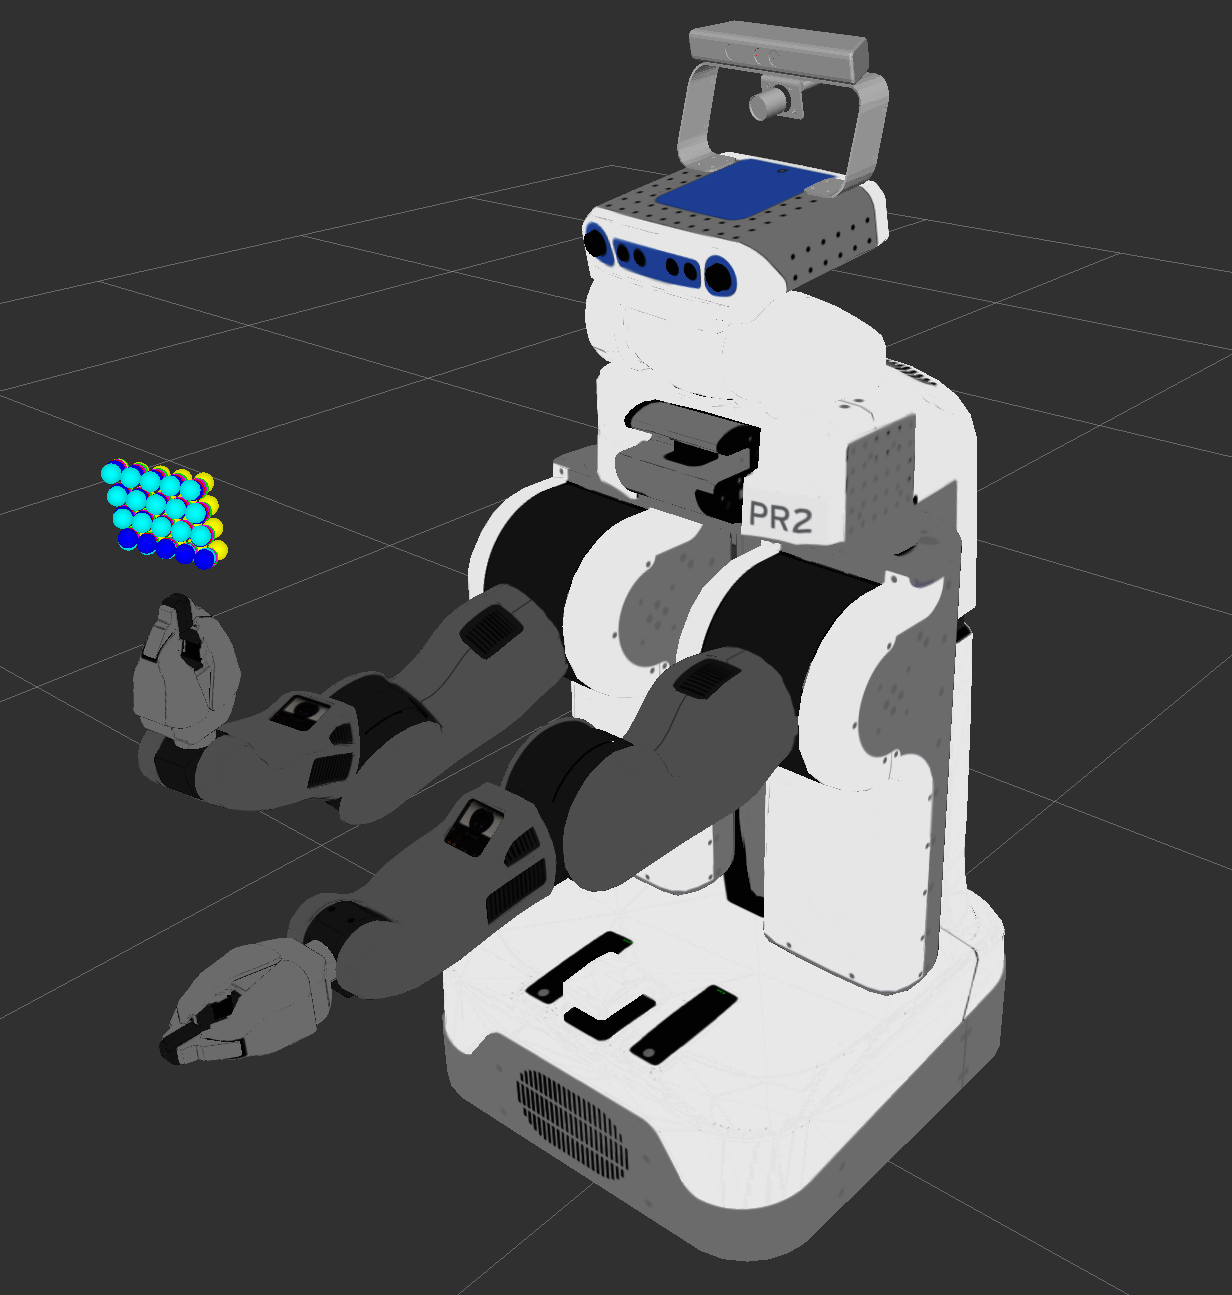
\includegraphics[height=0.25\textheight]{images/screenshots/calib08_1.png}
   }
 \caption{Checkerboard in hand.}
 \label{fig:cal_hand}
\end{figure}


\begin{figure}[!htbp]
 \centering
   \subfigure[Before estimation.]
   {
      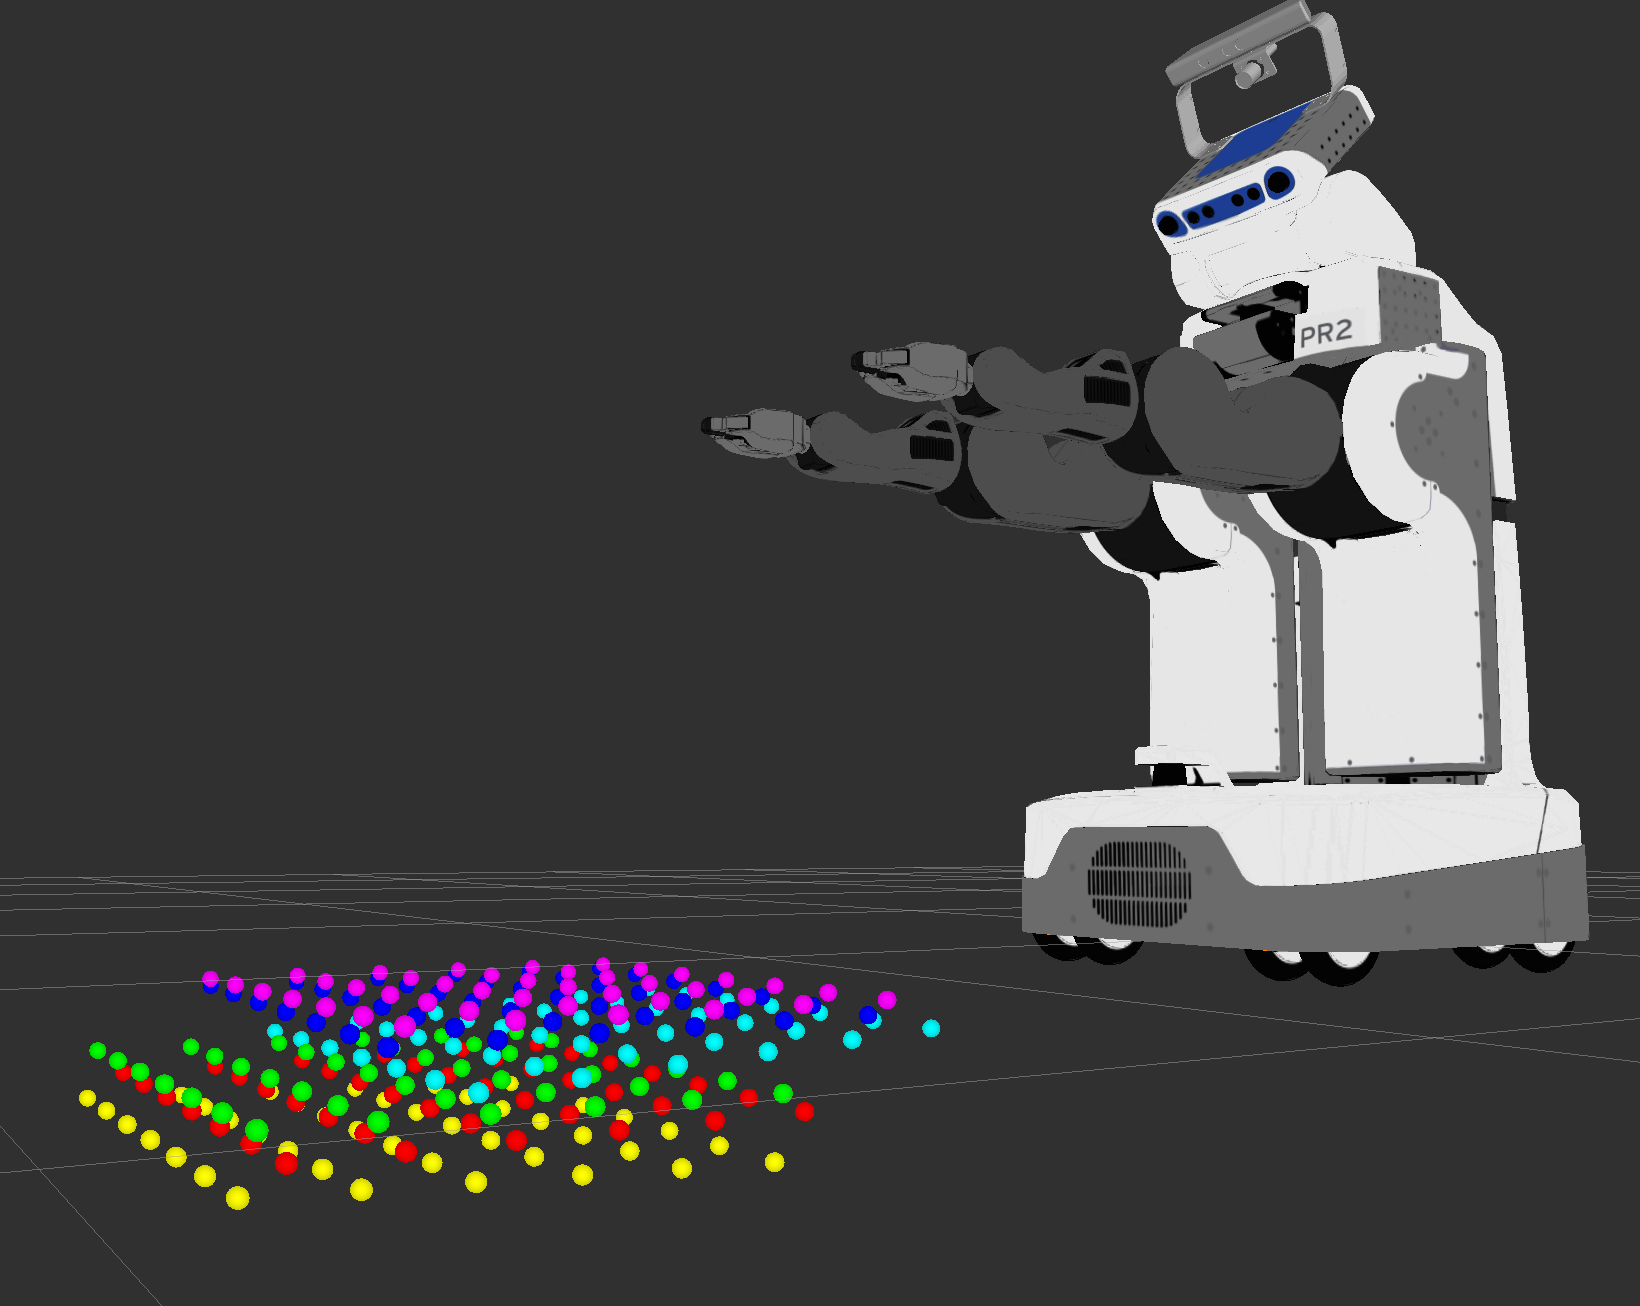
\includegraphics[height=0.25\textheight]{images/screenshots/uncal01_1.png}
   }
   \subfigure[After estimation.]
   {
      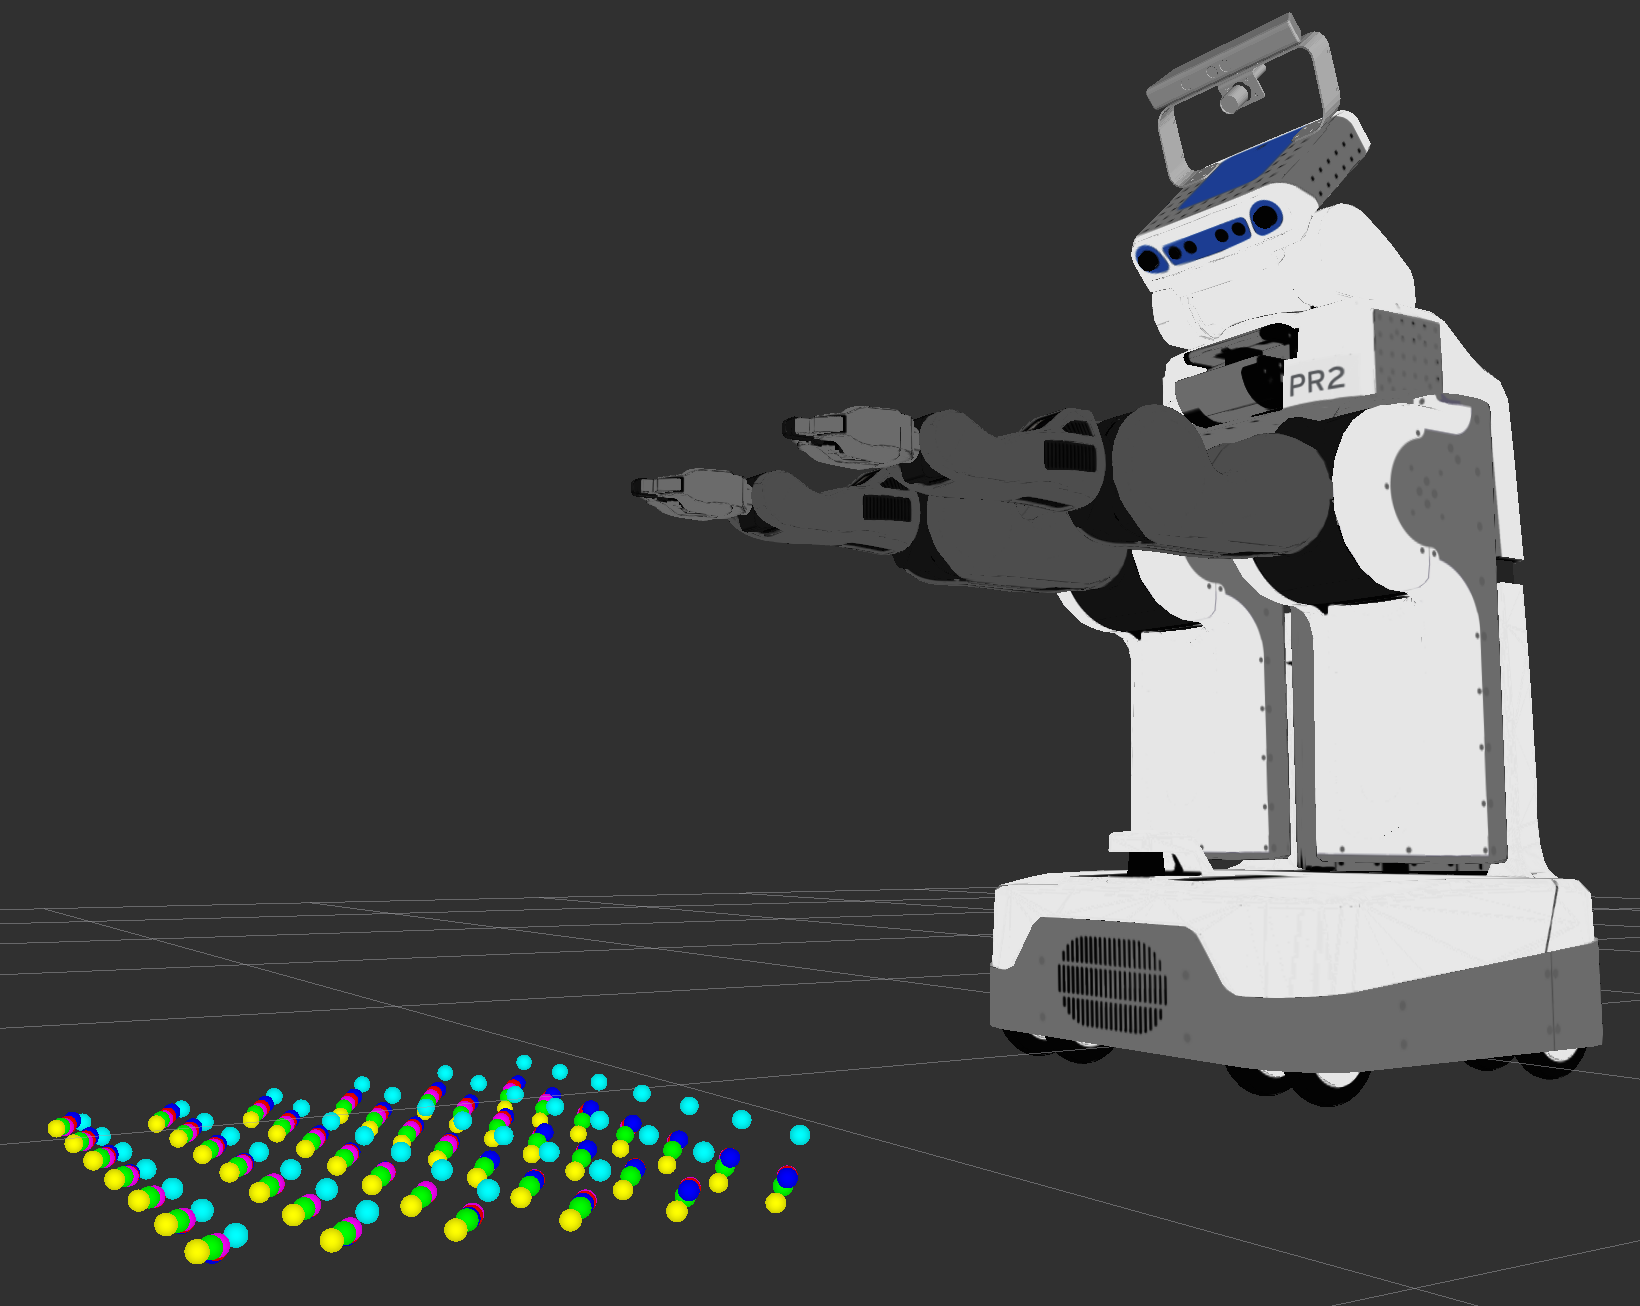
\includegraphics[height=0.25\textheight]{images/screenshots/cal01_1.png}
   }
 \caption{Checkerboard free in the world.}
 \label{fig:cal_free}
\end{figure}

\textbf{Note}: one of the camera does not show a good result (specially in Figure \ref{fig:cal_free}), corresponded to the prosilica camera, and a probable factor of this problem will be mentioned in the next section.


\subsubsection{Quantitative results}

As is mentioned above, the only finished implementation is the one which use solvePnP to find 3D points in the first camera (reference camera), and using those points as initialization for the structure. It is not an optimal solution and arise with a bias on the reference camera (\texttt{narrow\_left\_rect}): it has an excellent re-projection for the first camera in comparison with rest, as is perceived in Figure \ref{fig:boxplot_stats}.
% \begin{figure}[!htbp]
%  \centering
%  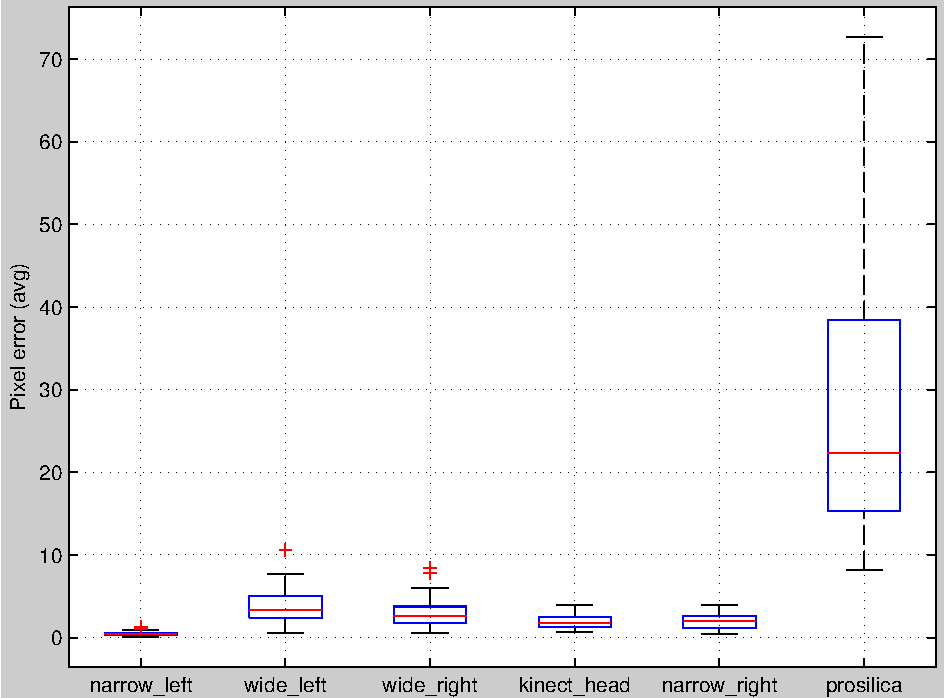
\includegraphics[width=0.35\textwidth]{images/boxplot_stats.pdf}
%  \caption{Visible bias in the first camera}
%  \label{fig:boxplot_stats}
% \end{figure}

\begin{figure}[!htbp]
 \centering
   \subfigure[With \texttt{prosilica} camera]
   {
      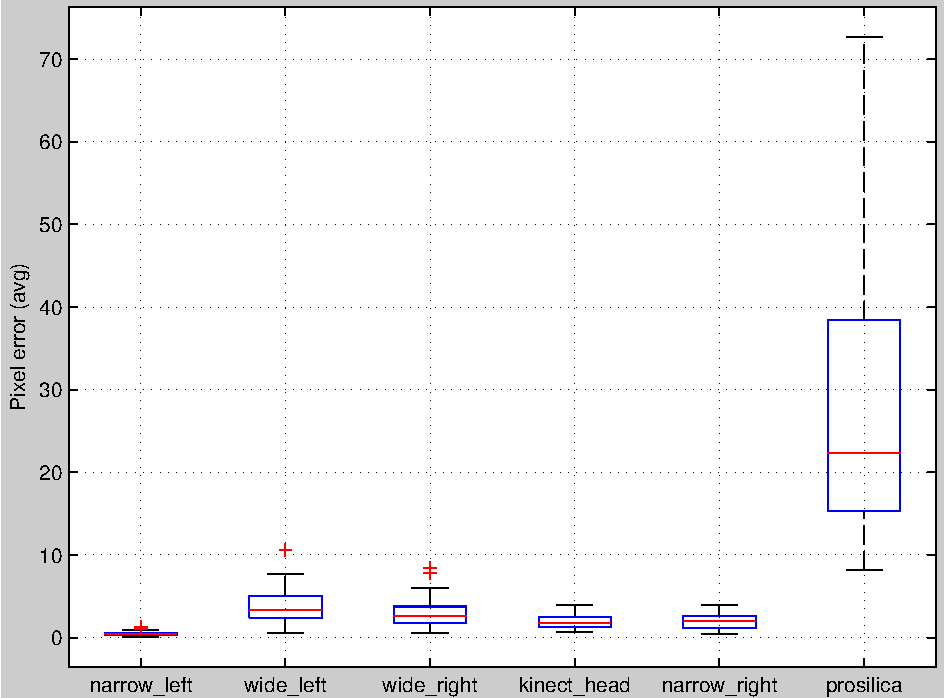
\includegraphics[height=0.25\textheight]{images/boxplot_stats.pdf}
      \label{fig:boxplot_stats}
   }
   \subfigure[Without \texttt{prosilica} camera]
   {
      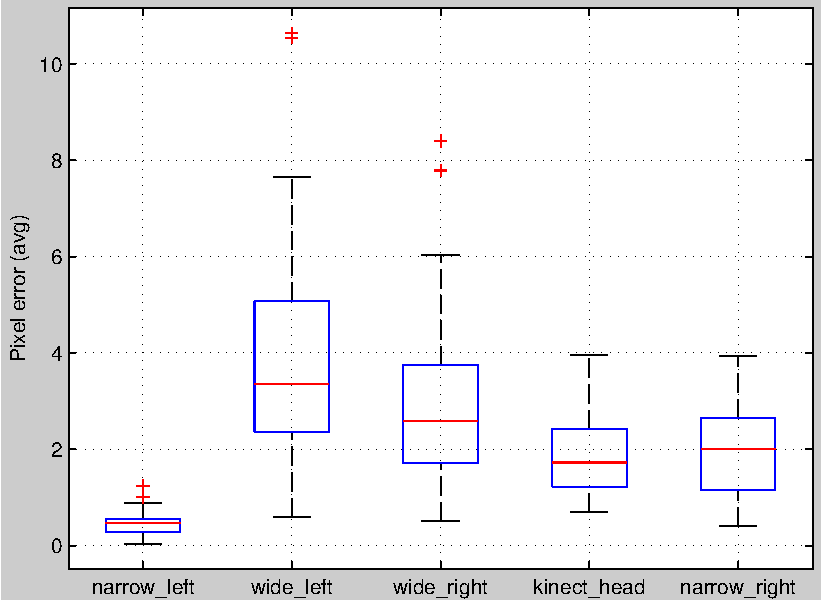
\includegraphics[height=0.25\textheight]{images/boxplot_stats_without_prosilica.pdf}
      \label{fig:boxplot_stats_without_prosilica}
   }
 \caption{Visible bias on first camera (with and without \texttt{prosilica} camera)}
%  \label{fig:boxplot_stats}
\end{figure}

In addition, it is possible to observe the \texttt{prosilica} camera has a bigger error than the remaining cameras. A wrong intrinsic calibration could be the reason. In order to determine if the bias was produced for this camera, same comparison has been repeated without taking into account the \texttt{prosilica} camera in the estimation process (Figure \ref{fig:boxplot_stats_without_prosilica}). Even though the global re-projection improves in this case, the bias continues on the first camera.




A visible comparison of this bias can been noted in Figure \ref{fig:reprojection}, where reprojected points after optimization are plot for two cameras: \texttt{wide\_left\_rect} and \texttt{narrow\_left\_rect} camera.
\begin{figure}[!htbp]
  \centering
    \subfigure[\texttt{wide\_left\_rect} camera]
    {
      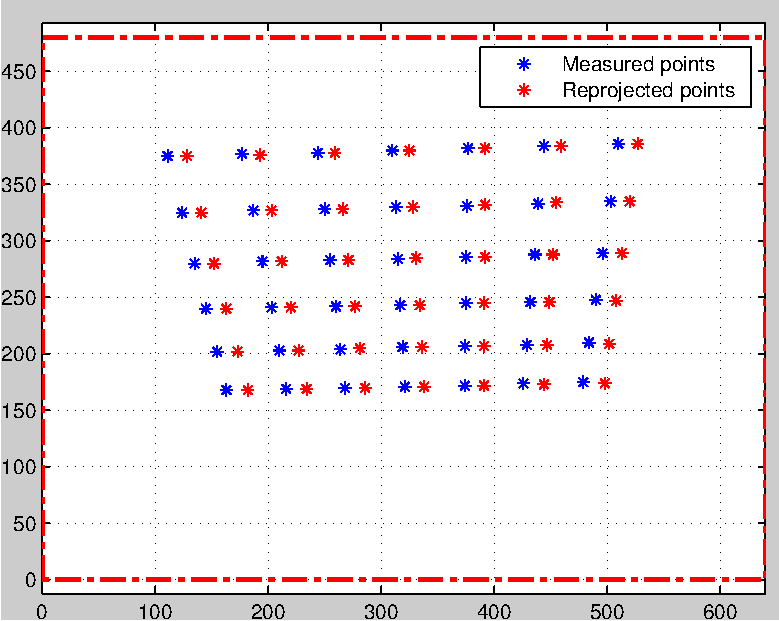
\includegraphics[width=0.45\textwidth]{images/reprojection02.pdf}
      \label{reprojection02}
    }
  \subfigure[\texttt{narrow\_left\_rect} camera (reference cam.)]
  {
    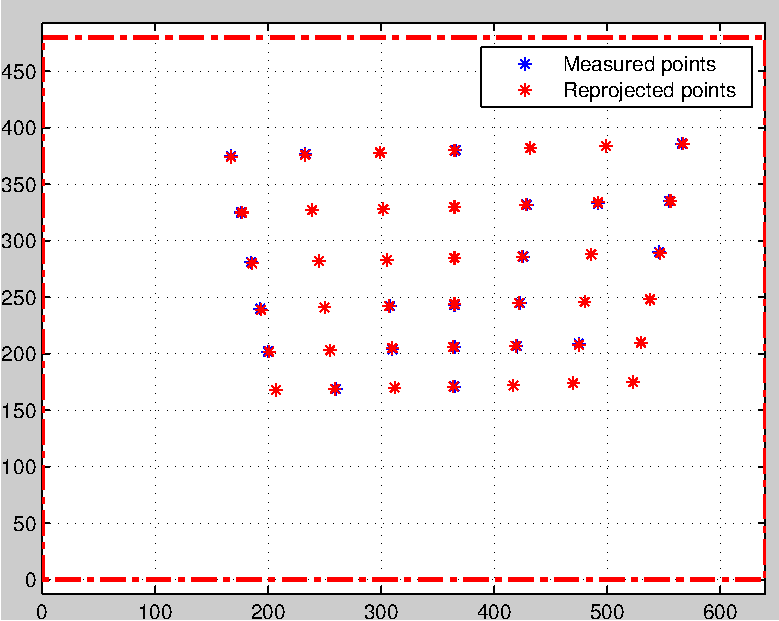
\includegraphics[width=0.45\textwidth]{images/reprojection01.pdf}
    \label{reprojection01}
  }
  \caption{Re-projection error after optimization}
  \label{fig:reprojection}
\end{figure}



More statistics (median, mean and standard deviation) can be observed in Figure \ref{fig:stats}.
\begin{figure}[!htbp]
 \centering
 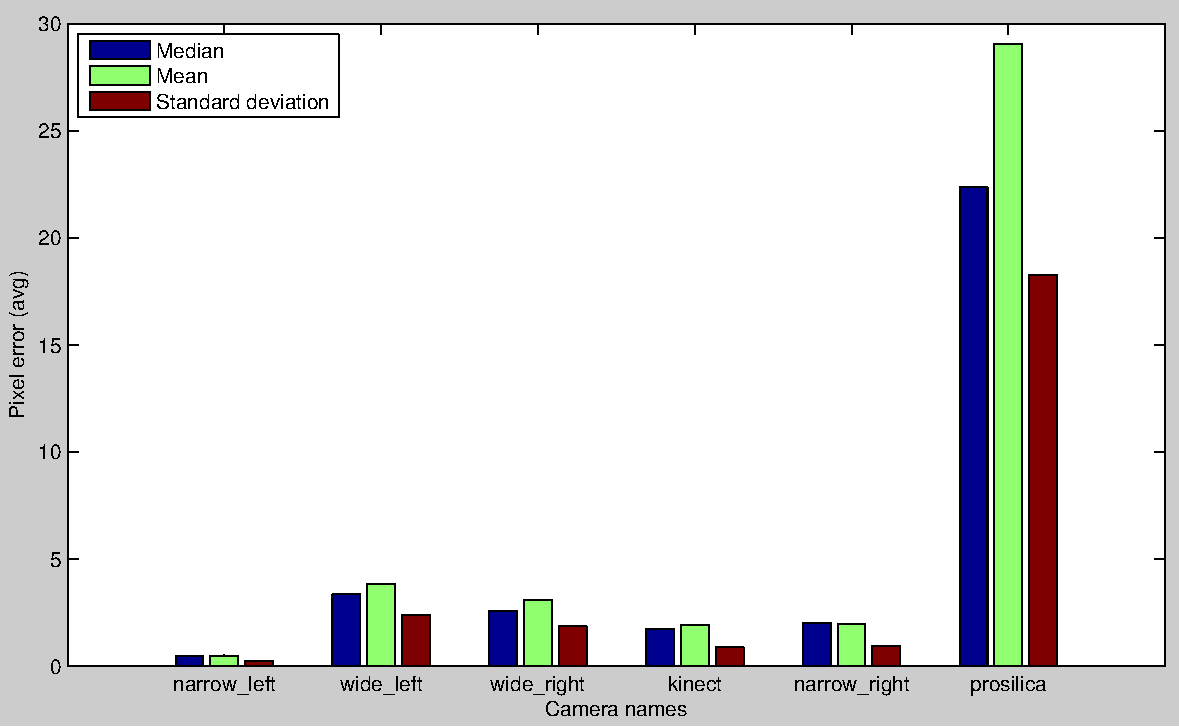
\includegraphics[width=0.65\textwidth]{images/stats.pdf}
 \caption{Median, mean, std after optimization}
 \label{fig:stats}
\end{figure}


Speed was not a priority goal of this project, but worth to mention that Ceres Solver takes few seconds to compute the result and less than 50 iteration to converge.




\chapter{Some implementation details}
\label{cha:implementation}

Software engineering decisions, problems, solutions?, and resignations... :P


----

Why re-implement the calibration estimation package?

Why re-implement the robot\_state\_publisher? Explain the how to Publish the /tf tree?
Y porque cuando se actualizaba empezaba a danzar, por los 0.5 seg. de retraso en los fixed links.
Why KDL? KDL structures are not modificable, so it was needed to re-create KDL once the urdf is updated.

RViz and Markers! Republish everytime!

% \subsection{}
* Quaternions: used to avoid singularities...

* Data/Views in different order... explain... some views aren't visible for all the cameras.

(optional)
Why Ceres?




\section{Code}
\subsection{Cost function}
\label{sec:ceres_impl}


% \section{...}

\subsection{Creating model point for solvePnP}
\label{sec:solvePnP_impl}
It is was necessary to create a function that


\section{Fails and solutions}

Explain why it fails
\begin{figure}[!htbp]
 \centering
 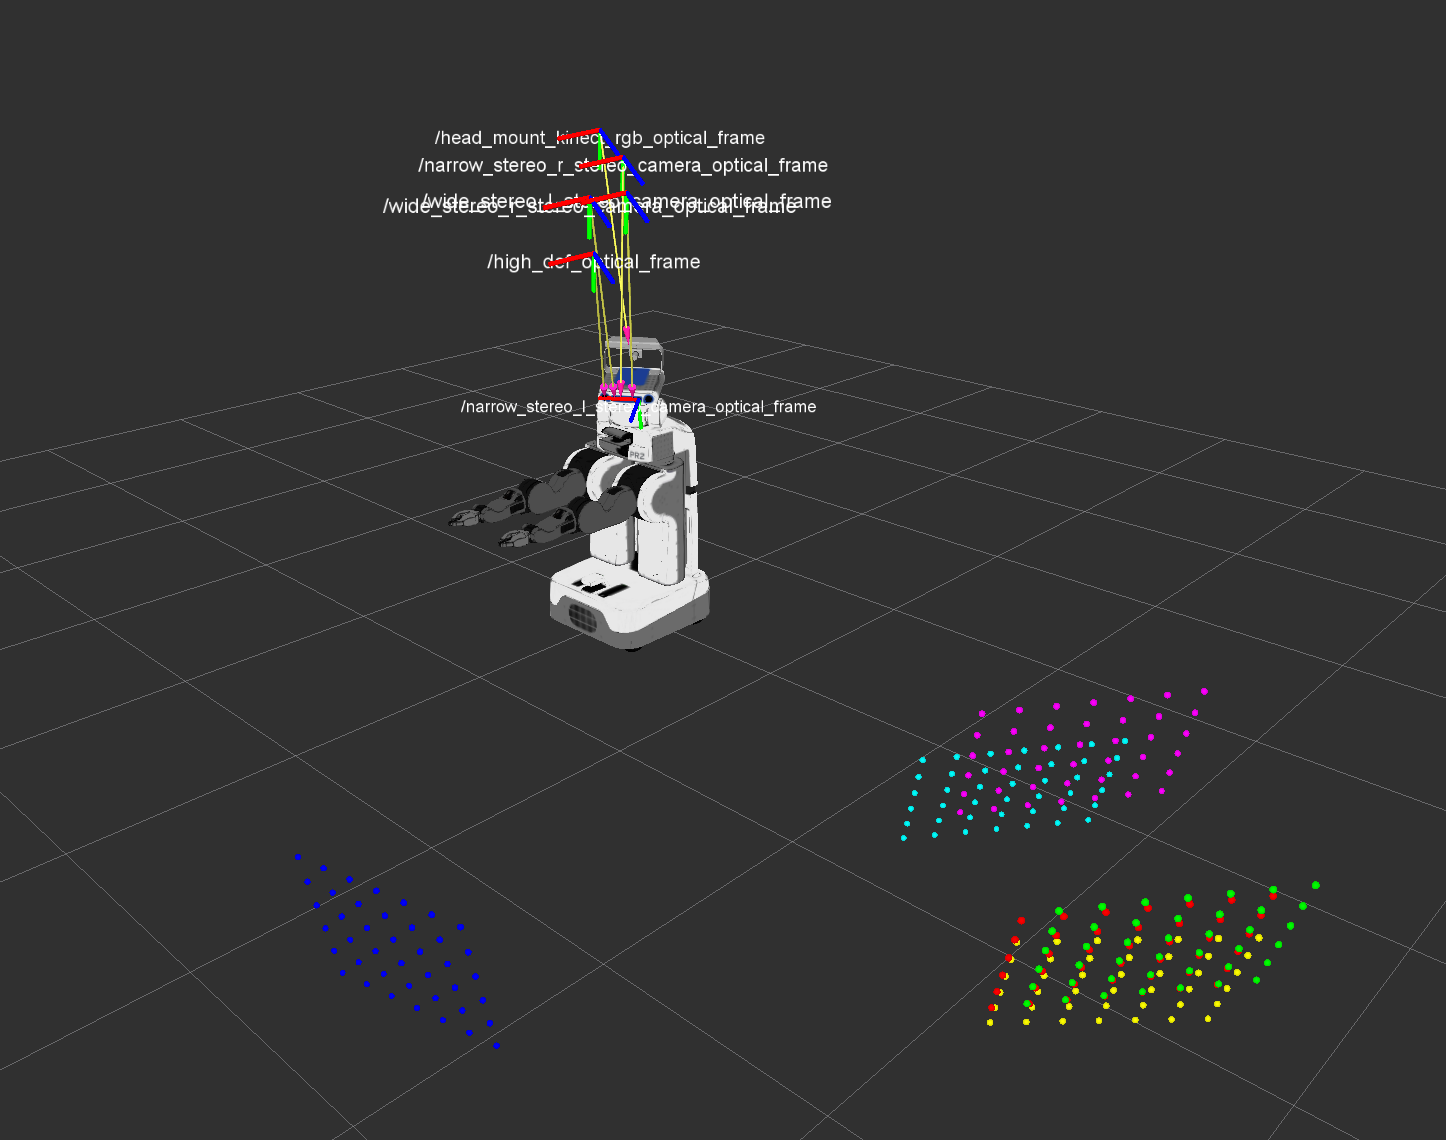
\includegraphics[width=0.5\textwidth]{images/screenshots/optimization_failer02_2.png}
 \caption{Initials versions}
 \label{fig:optimization_failer}
\end{figure}


Triangulation fails... no solution in the moment of writing this thesis :( I couldn't find the bug
\begin{figure}[!htbp]
 \centering
 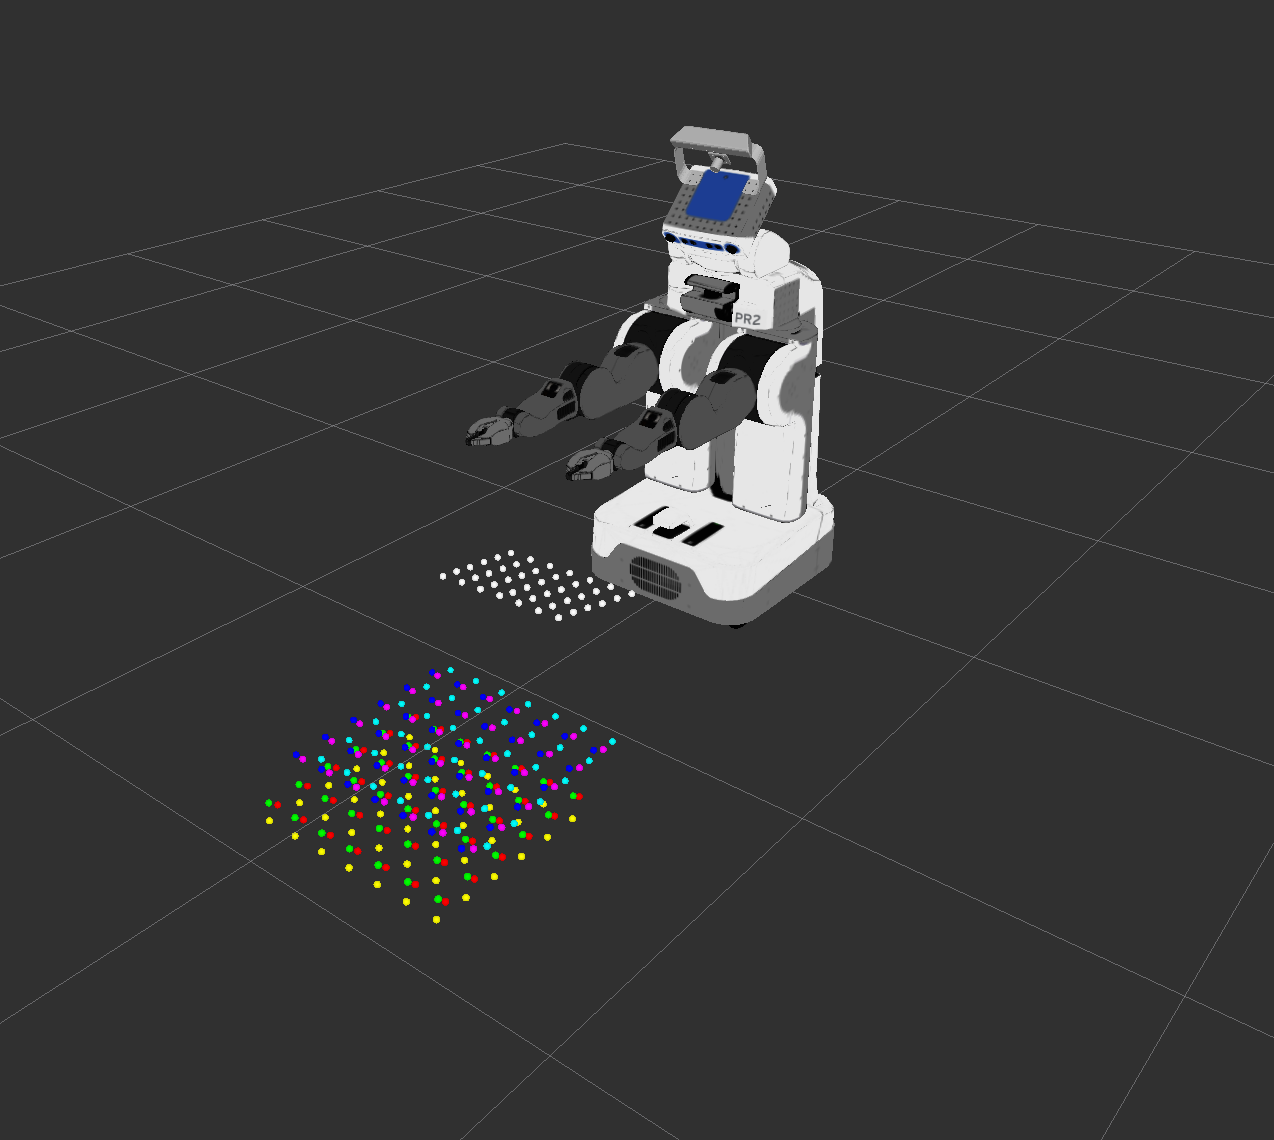
\includegraphics[width=0.5\textwidth]{images/screenshots/triangulation_fails.png}
 \caption{Triangulation fails, white dots}
 \label{fig:triangulation_fails}
\end{figure}




\chapter{Extra work}
\label{cha:extra}

(this chapter is more than optional)

Work not related to the thesis, but time consuming, like commits in Ceres, fixed bugs in URDF dom (export\_urdf() function), etc...



\chapter{Future work}
\label{cha:future}

ideas and all the things I didn't finish but I supposed to... :P

\chapter{Future work}
\label{cha:future}

Since the ROS package describes in this thesis is still in development stage many things need to be improved, some points are listed here:

\begin{itemize}
 \item The highest priority is to fix triangulation in order to get a better structure initialization, this will lead to a considerable improvement in the whole calibration system.


 \item User interface is required to make the package more useful.

 \item The system should be robot agnostic. There is a wizard in the new Moveit! package that can be used it to create the configuration files.

 \item Export the URDF to a file. I had to fixed some bugs in the URDF Dom package, they will allow to create this functionality.

 \item Validate the proposed method in chapter \ref{cha:additional} for motion initialization.

\end{itemize}


\chapter{Conclusions}
\label{cha:conclusions}

This project combines the strongest of several \textbf{open-source} components: KDL, Ceres Solves, ROS, OpenCV and PR2 (open-source platform, see Figure \ref{fig:PR2_free_robot}). It cannot be less to contribute in the same way to the community, making the code freely available as a ROS package (even though it is still in development stage).

\begin{figure}[!htbp]
 \centering
 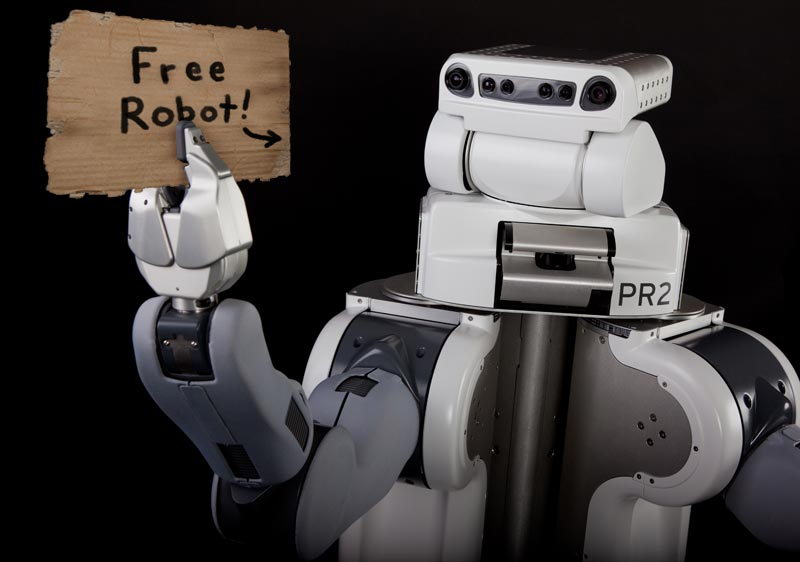
\includegraphics[width=0.65\textwidth]{images/PR2_free_robot.jpg}
 \caption{PR2 pleased to be free.}
 \label{fig:PR2_free_robot}
\end{figure}

The above mentioned software components are well designed, with excellent interfaces and documentation. Even though this fact, \textbf{combining} them in an unique product is a \textbf{time consuming} task, which requires different type of abilities; for example, solve compilation problems with CMake or Catkin (new compilation system in ROS), to mention one.

Regarding the thesis itself, \textbf{robot calibration} is an important problem to be solved in any robot, in order to allow an effective interaction with the environment. And this thesis has been focused in \textbf{multiple camera calibration}. The work has been done by experimenting with real data, real robots, real problems.

Two different methods have been proposed for the \textbf{structure initialization} (3D points). Initialization used for the bundle adjustment optimizer (Ceres Solver). These methods are: solvePnP --3D points in the camera reference-- and n-view triangulation method.

The improvement in calibration has been shown \textbf{visually} --for a human-friendly comparison-- and \textbf{quantitatively} --for a more rigorous analysis--. A bias has been observed in the solvePnP solution, which will lead to future research with the aim to improve results using n-view triangulation method. %, with the intention of improve the results even more.

In addition to the practical experimentation, a theoretical development has been also elaborated in the framework of epipolar geometry, in which a method for motion initialization is discussed.


To conclude with this thesis, it has been a \textbf{proud} to work with two excellent person like David Fofi and Vincent Rabaud, in two excellent places like Le2i and Willow Garage.



% \appendix
% \chapter{Lemma demonstrations}
\label{ap:proof}

This Appendix has auxiliary lemmas used in the theorem (\ref{th:norm}) proof. Knowledge of linear algebra will be assumed.

% \cite{Strang:1993}

\begin{lemma}
\label{lemma:symmetric}
\[ \left.
  \begin{array}{l}
  A = Q\,\Lambda\,Q^T \\
  \Lambda \mbox{ diagonal matrix} \\
  Q \mbox{ symmetric matrix}
  \end{array} \right\}
  \Rightarrow
  A \mbox{ and } \Lambda \mbox{ have same eigenvalues.}
\]
\end{lemma}

\begin{proof} See \cite{Strang:1993} for a demonstration.
\end{proof}


\begin{lemma}
\label{lemma:singular_values}
\[ \left.
  \begin{array}{l}
  E =[t]_{\times}R \\
  ||t||=k
  \end{array} \right\}
  \Rightarrow
  E \mbox{ has two singular values equal to $k$ and the last one is zero.}
\]
\end{lemma}

\begin{proof}
From \cite[Result A4.1 (ii)]{HZ2},
\begin{align*}
S=[t]_{\times} \mbox{ is skew-symmetric } & \quad\Rightarrow\quad S = \alpha\,U\,Z\,U^T, \quad \mbox{ with $U$ orthogonal} \\
        &  \quad\Rightarrow\quad  S = U\,Z_{\alpha}\,U^T
\end{align*}
where
\begin{equation}
Z =
\begin{pmatrix}
  0 & 1  & 0 \\
 -1 &  0  & 0 \\
  0 &  0  & 1
\end{pmatrix}, \quad\quad\quad
Z_{\alpha} =
\begin{pmatrix}
  0 & \alpha  & 0 \\
 -\alpha &  0  & 0 \\
  0 &  0  & 1
\end{pmatrix}
\end{equation}
Taking
\begin{align}
S\,S^T & = U\,Z_{\alpha}\,U^T (U\,Z_{\alpha}\,U^T)^T \nonumber \\
       & = U\,Z_{\alpha}\,(U^T U)\,Z_{\alpha}^T\,U^T \nonumber \\
       & = U\,Z_{\alpha}\,Z_{\alpha}^T\,U^T \label{eq:similar_matrix}
\end{align}
From (\ref{eq:similar_matrix}),
\begin{align}
S\,S^T \mbox{ and } Z_{\alpha}\,Z_{\alpha}^T \mbox{ are similar matrices } & \quad\Rightarrow\quad tr(S\,S^T) = tr(Z_{\alpha}\,Z_{\alpha}^T) \label{eq:equal_trace}
\end{align}
By expansion,
\begin{equation}
S\,S^T =
\begin{pmatrix}
  t_3^2 + t_2^2 & 0  & 0 \\
  0 &  t_1^2 + t_3^2  & 0 \\
  0 &  0  & t_2^2 + t_1^2
\end{pmatrix}
\end{equation}
then,
\begin{equation}
\label{eq:S_trace}
tr(S\,S^T) = (t_1^2 + t_2^2 + t_3^2) + (t_1^2 + t_2^2 + t_3^2) = 2\,||t||^2 = 2\,k^2
\end{equation}
In the other hand (by expansion),
\begin{equation}
\label{eq:Z_trace}
tr(Z_{\alpha}\,Z_{\alpha}^T) =
tr\,\begin{pmatrix}
  \alpha^2 & 0  & 0 \\
  0 &  \alpha^2  & 0 \\
  0 &  0  & 0
\end{pmatrix} = 2\,\alpha^2
\end{equation}
From (\ref{eq:similar_matrix}), (\ref{eq:S_trace}) and  (\ref{eq:Z_trace}),
\begin{equation}
\alpha^2 = k^2
\end{equation}
and also
\begin{equation}
\label{eq:ZZT}
Z_{\alpha}\,Z_{\alpha}^T =
\begin{pmatrix}
  k^2 & 0  & 0 \\
  0 &  k^2  & 0 \\
  0 &  0  & 0
\end{pmatrix}
\end{equation}
Now, since $Z_{\alpha}\,Z_{\alpha}^T$ diagonal, and $U$ is orthogonal (symmetric), it is possible to use lemma (\ref{lemma:symmetric}) then,
\begin{equation}
\label{eq:SST_same_ZZT}
\mbox{$S\,S^T$ has the same eigenvalues than $Z_{\alpha}\,Z_{\alpha}^T$}
\end{equation}

\begin{center}
\line(1,0){250}
\end{center}

Now, we start from the hypothesis:
\begin{align}
\label{eq:EET_same_SST}
E=S\,R & \quad\Rightarrow\quad E\,E^T = S\,R\,(S\,R)^T = S\,R\,R^T\,S^T = S\,S^T
\end{align}
From (\ref{eq:SST_same_ZZT}) and (\ref{eq:EET_same_SST}),
\begin{equation}
\label{eq:EET_same_ZZT}
\mbox{$E\,E^T$ has the same eigenvalues than $Z_{\alpha}\,Z_{\alpha}^T$}
\end{equation}
Then,
\begin{equation}
E \mbox{ has two singular values equal to $k$ and the last one is zero.}
\end{equation}
and,
\begin{equation}
E = U\, diag(k,k,0)\,V^T            \quad\quad\mbox{a SVD decomposition}
\end{equation}


\end{proof}





%   this is for BibTeX.  remove if you plan to write the references in the document
\bibliographystyle{unsrt}
\bibliography{refs}


%adds the bibliography to the table of contents
\addcontentsline{toc}{chapter}
         {\protect\numberline{Bibliography\hspace{-96pt}}}

\end{document}
